% Template for PLoS
% Version 1.0 January 2009
%
% To compile to pdf, run:
% latex plos.template
% bibtex plos.template
% latex plos.template
% latex plos.template
% dvipdf plos.template

\documentclass[10pt]{article}

% amsmath package, useful for mathematical formulas
\usepackage{amsmath}
\setcounter{MaxMatrixCols}{50}
% amssymb package, useful for mathematical symbols
\usepackage{amssymb}

% graphicx package, useful for including eps and pdf graphics
% include graphics with the command \includegraphics
\usepackage{graphicx}

\usepackage{bussproofs}

% cite package, to clean up citations in the main text. Do not remove.
\usepackage{cite}

\usepackage{color}

% Use doublespacing - comment out for single spacing
%\usepackage{setspace}
%\doublespacing

% Text layout
\topmargin 0.0cm
\oddsidemargin 0.5cm
\evensidemargin 0.5cm
\textwidth 16cm
\textheight 21cm

% Bold the 'Figure #' in the caption and separate it with a period
% Captions will be left justified
\usepackage[labelfont=bf,labelsep=period,justification=raggedright]{caption}

% xy-pic for diagrams
\usepackage[all]{xy}
% subcaption
\usepackage{subcaption}
% hyperref
\usepackage{hyperref}
% color table cells http://goo.gl/ZmpJv
\usepackage[table]{xcolor}
% rotate text in table http://goo.gl/Lb4Zd
\usepackage{rotating}
% listings for code highlighting in appendix
\usepackage{listings}
\usepackage{setspace}
\input{tex/listingspython}
\usepackage{placeins}

%define colors
\definecolor{DeepRed}{rgb}{.82,.14,.16}
\definecolor{DeepBlue}{rgb}{0,0.36,0.62}

% Use the PLoS provided bibtex style
\bibliographystyle{plos2009}

% Remove brackets from numbering in List of References
\makeatletter
\renewcommand{\@biblabel}[1]{\quad#1.}
\makeatother


% Leave date blank
\date{}

\pagestyle{myheadings}
%% ** EDIT HERE **


%% ** EDIT HERE **
%% PLEASE INCLUDE ALL MACROS BELOW

%% END MACROS SECTION


\begin{document}

% Add Figure, Table prefixes to references
% http://tex.stackexchange.com/a/6063/6784
\let\ref\autoref

% Table of contents
% http://tex.stackexchange.com/a/7357/6784
%\pagebreak
\pagenumbering{gobble}
\tableofcontents
\listoffigures
\listoftables
\pagebreak
\pagenumbering{arabic}

% Title must be 150 characters or less
\begin{flushleft}
{\Large
\textbf{Modularization of global genotype-phenotype mappings accesses a relative superset of biological functions}
}
% Insert Author names, affiliations and corresponding author email.
\\
Cameron Smith$^{1}$,
Ximo Pechuan$^{1}$,
Daniel Biro$^{1}$,
Aviv Bergman$^{1,2,3,4, \ast}$
\\
\bf{1} Department of Systems and Computational Biology,
\bf{2} Dominick P. Purpura Department of Neuroscience,
\bf{3} Department of Pathology, Albert Einstein College of Medicine, Bronx, NY, USA
\bf{4} Santa Fe Institute, 1399 Hyde Park Road, Santa Fe, NM 87501, USA
\\
$\ast$ E-mail: aviv@einstein.yu.edu
\end{flushleft}

% Please keep the abstract between 250 and 300 words
\section{Abstract}
%!TEX root = ../plos_template.tex
Different gene regulatory network architectures are commonly thought to provide access to different collections of gene expression patterns that may ultimately result in different phenotypes~\cite{Alon2007}. The manner in which stochasticity in the gene expression process~\cite{Eldar2010,Sanchez2013} impacts the relationship between network architecture and the expression patterns each is capable of producing is not clear~\cite{Jothi2009,Chalancon2012}. In order to investigate this relationship, we begin with the finest grained notion of genotype to phenotype map, gene expression, and adopt a formalism to reason generally about probability distributions over such maps~\cite{Lane1998,MacLane1992,Awodey2006,Abramsky2011}. In all cases, this must be relative to a notion of network architecture, defined here as a hypergraph determining a hierarchical model~\cite{Lauritzen1996} over a given set of genes. We show that in a simple case where the highest-order gene regulatory interactions are allowed, then under some conditions the collection of accessible phenotypes is smaller than in some of the alternative cases in which only lower-order interactions are allowed. This conclusion is arrived at by comparing the geometries of spaces of probability distributions on genotype-phenotype maps for the case of a genome containing a given number of simultaneously interacting genes to the equivalent for all of the other possible gene regulatory network topologies on the same number of genes. We find that the latter spaces of probability distributions associated to the restriction to lower-order interactions are actually larger than the former one whenever the gene regulatory network topology contains a cyclic structure. A generalization of this result to an arbitrary number of genes implies that modularization of interactions, defined here as restriction from relatively higher- to lower-order interactions, within and among gene regulatory networks permits access to additional correlation patterns of expression among multiple interacting genes. That these additional gene expression patterns may enable the fulfillment of functional requirements in certain environments while remaining intrinsically inaccessible when highest-order interactions are allowed implies that, even when gene expression stochasticity is taken into account, network architectures may be functionally differentiated and thus serve as substrate for natural selection in a background of otherwise evolutionarily neutral space. The identification of \emph{interaction constraint}~\cite{Bar-Even2006,Johnson2010a} as an enabler as opposed to a limitation on accessible phenotypes may contribute to a more general explanation for the hierarchical modular architecture~\cite{Ravasz2002,Segre2005,Wagner2007,Erwin2009,Jothi2009,Bhardwaj2010,Colm} of the gene regulatory networks observed throughout the tree of life.


% Please keep the Author Summary between 150 and 200 words
% Use first person. PLoS ONE authors please skip this step.
% Author Summary not valid for PLoS ONE submissions.
%\section{Author Summary}
%%!TEX root = ../plos_template.tex
Several broadly applicable features of gene regulatory networks have been identified and experimentally validated to a reasonable level of confidence in the past few decades. Among these features are 1. stochasticity in the transcription process and 2. hierarchical modularity in gene regulatory network architecture. In this study, we consider explanations for the interplay between these two important features in a semi-formal model that considers both the developmental and evolutionary processes. We demonstrate within the context of our stylized model that the space of all possible gene expression patterns should be considered relative to a gene regulatory network architecture. Furthermore, we present a method that can in principle quantify these relationships for gene regulatory networks of arbitrary topological structure. This recognition derives from and has important future implications for the development of a constraint-based approach to characterizing the coevolution of stochasticity and hierarchical modularity and to modeling evolutionary processes more generally.


\section{Introduction}
%!TEX root = ../plos_template.tex
Probabilistic models of gene regulation serve as a bridge between theory and experiment.  On the one hand, parameters in a probabilistic model can be fit to data obtained by measuring gene expression using microarray or sequence census methods \cite{Friedman2008a,Zhang2013}.  On the other hand, one can model a genetic network as a deterministic or stochastic reaction network which tracks levels of molecules at the nucleic acid or protein level \cite{Alon2006,Voit2012}.  From the solution to this latter kind of model, one can then obtain theoretical predictions for the parameters of the probabilistic model in terms of reaction rates.  Comparison of the parameters fitted from data with the predicted values serves as a means for comparing theory with experiment and can serve as a starting point for improving the theory or for designing future experiments \cite{Tonsing2014}.

An important feature of experimental science is that it involves partial information.  In the course of a single measurement, one typically is not able to observe a biological network in its entirety.  Rather, one observes a subnetwork at a time and only obtains a more complete picture by later combining these partial views.  This contrasts with theory, where, one makes a representation of a closed system that provides explicit values for all quantities of interest.  In order for a probabilistic model to serve its purpose, it should also accomodate partial information and thus we will explicitly consider the effects of 1) carving out a subnetwork from its context and 2) coarse-graining observables. Observables representing partial information will generally arise in situations where a system is interacting with another system. This situation arises in the context of interpreting gene expression data as well as in the interactions of an organism's gene regulatory network with the organism's environment.

% Studying this situation, we find that instances arise where the fact that a network context may interact with only partial information of the states of a given subnetwork can result in apparent inconsistency. Furthermore,

Inconsistency arises when a network context places more constraints on a network than it is capable of satisfying. One of the canonical examples of this arose in the study of ferromagnetism via the Ising model on a triangular lattice where so-called \emph{frustration} arises among the couplings of three nearest-neighbor spins \cite{Wannier1950,Toulouse1977,Vannimenus1977}. We exhibit a method of checking for such consistency and evaluating its likelihood of arising in the context of building probabilistic models of gene regulatory networks. When apparent inconsistency is observed, it must arise from the network context interacting with only partial information of the states of a given subnetwork. This would indicate that information about the network context must be included in order to maintain a consistent model of the system.

Consider the case in which the network context is an environment placing independent and identical functional requirements upon a population of similar independent subnetworks and selecting for their architectures over many generations to satisfy those requirements. Our analysis of the probability of inconsistency arising relative to network architecture demonstrates that networks with a larger number of cycles are more likely to be subjected to inconsistent constraints that will be unable to be jointly satisfied. Since this probability of inconsistency is higher for networks with a larger number of cycles, this results in implicit selection against regulatory network architectures with a larger number of cycles. One would not expect such a bias to eliminate the existence of cycles in gene regulatory networks. However, it is reasonable to expect on the basis of this result a kind of hierarchical modularity: where modules that may possess cycles and are small relative to the overall size of the network exist within a globally hierarchical network structure. A similar problem has been considered previously in the context of population genetics \cite{EthanAkin389}. Of course, there are other factors which may contribute to the development of such network architectures. The evaluation of the hierarchical modularity property will require extensive future work, but its existence is consistent with many studies that have evaluated the architecture of gene-regulatory networks~\cite{Ravasz2002,Segre2005,Wagner2007,Erwin2009,Jothi2009,Bhardwaj2010,Chalancon2012,Colm}.

We explain the connection between stochastic process models of gene expression and \gnpm{} in \ref{sec:genenetworkphenmap}. \ref{sec:probabilitydistributionsonnetworks}--\ref{sec:compatibilityofgpms} contain the underlying mathematical justification for our claims, and they can be skipped by those who are primarily interested in the implications of our results. In \ref{sec:probabilitydistributionsonnetworks} we introduce the concept of network modules and define probability distributions over their expression states. We describe how one can pass from expression states to more coarse-grained phenotypes such as the ability to produce a given metabolite in a manner that is dependent upon interactions among multiple genes in \ref{sec:coarsegrainingphenotypes}. In \ref{sec:covergenotypespace} we define a gene regulatory network architecture (GRNA) as a collection of subsets of genes that together comprise a larger set of genes. The different ways in which this is accomplished correspond to distinct GRNAs. \ref{sec:compatibilityofgpms} describes the different compatibility conditions that arise for different GRNAs and demonstrates how these compatibility conditions lead to a set of inequalities determining a space of probability distributions for each GRNA. \ref{sec:cycliccontextunsatisfiableconstraints} and \ref{sec:probconstrgeometry} examine these constraints for the example of the three-cycle GRNA. \ref{sec:volrat} computes the likelihood of unsatisfiable constraints for all GRNAs on four genes that possess cycles. Finally, \ref{sec:unsatisfiableconstrevolution} explains implications for the evolution of GRNA of the result that networks with a larger number of cycles are more likely to have unsatisfiable constraints placed upon them.

% Traditional dynamical models of gene-regulatory networks begin by treating them as reaction networks whose known or hypothesized interactions are encoded by sigmoidal response functions \cite{Alon2006,Voit2012}. Genes that interact do so in such a manner as to either activate or inhibit one another leading to a dynamical model of the gene expression process.
% \begin{eqnarray*}
% {dg_i \over dt} =
% k_{is}  \prod_{j=1}^{N} \frac{k_{ija} g_j^{n_{ija}}}{1+k_{ija} g_j^{n_{ija}}}
% \frac{1}{1+k_{ijr} g_j^{n_{ijr}}} - k_{id} g_i
% \end{eqnarray*}
% for a network of $N$ genes where $g_i$s represent concentrations of gene products, $k_{ija}$s represent activation rates, $k_{ijr}$s represent repression rates, and $k_{id}$s represent degradation rates.
% The dual perspective is taken by probabilistic models whose parameters are fit to data obtained by measuring gene expression using microarray or sequence census methods \cite{Friedman2008a,Zhang2013}.
% In both of these classes of models, higher-order correlations are assumed to be accurately represented in terms of a sum over lower-order correlations.

% The evolution of \gnpm{} is an open question in biology. Specifically, how the higher level constraints imposed upon a system at a phenotypic level shape the elements and the interaction among the elements at a lower, genotypic level. Here we neglect the specific mechanisms by which one achieves such phenotypes and assume a statistical view of the observed phenotype. This communication introduces a framework that enable us to analyze how higher-level constraints, formulated in terms of probability of gene expression pattern might shape the allowable interactions among elements at a lower level.

% The genotype of an organism has a relatively straightforward definition in terms of the sequence of nucleotides comprising its genome. Phenotypes, on the other hand, can be described at different levels of organization~\cite{Dawkins1982,Stadler2001}. The concept of phenotype was initially defined at the level of macroscopically observable physical characteristics such as shape, size, color, and various combinations thereof~\cite{Johannsen1911}. However, since the advent of molecular biology, the lowest level description of phenotype might be considered to be the dynamic phenomenon that can be described by measuring the transcription states of all genes comprising an organism's genome. The time series that results from such observations can be used to infer various statistics that characterize gene expression such as correlations between pairs of genes. The statistics associated to any higher-level phenotype that is determined by a particular gene expression pattern should be functions of such statistics.

% % The present capability to observe phenotypes at various levels of organization raises several questions about \gnpm{}. One is how to define and characterize properties of the fundamental level of \gnpm{} that is embodied in the transcription process. Another is how to define and characterize the manner in which higher-order ``phenotype$_i$-phenotype$_{i+1}$'' mappings built on top of this one are affected by the properties of each of the levels existing below, and, on evolutionary timescales over which feedback may play a significant role, potentially also those above it.

% % We attempt to address these questions from an abstract perspective that is independent of the particular physical implementation of \gnpm{} in terms of complex networks of molecular interactions.
% We present a formal probabilistic description of the \gnpm{} that takes into account higher-order correlations among genes as well as evidence that gene expression is stochastic \cite{Swain2002,Paulsson2004,Thattai2004,Acar2008a,Lestas2010,So2011,Munsky2012,Neuert2013,Sanchez2013}. In order to assess the impact of these features on the evolution of gene regulatory network architecture, where architecture is here considered to be determined exclusively by observable correlations among genes \cite{Friedman2008a}, we use this description to precisely pose the question: For any genotype, given a space of probability distributions on the collection of \gnpm{}, does modularization of the genotype (restriction of correlations among genes, \refsupp{}) increase, decrease, or leave invariant the size of the accessible space of selectable gene expression patterns?
% % For example, if we have three genes that can all participate in a higher-order interaction (the highest-order among three genes being a trinary interaction) that generates a phenotype, but we restrict interactions to a lower-order subset consisting of all three possible binary interactions then this represents one particular way of modularizing over a given genotype (compare \ref{fig:conediagram}B top and middle).

% For those cases in which modularization results in no change to the space of probability distributions over \gnpm{} with respect to that defined on the full genotype (i.e. the single highest-order correlation referred to as non-modular), then there may be no method to select for one network architecture over another. On the other hand any differences in gene expression patterns that result from differences in network architecture may allow certain network architectures to be selected relative to one another. Here we show that those modularizations that introduce cycles into the gene-regulatory network architecture also expose the capacity for negative selection as a result of additional restrictions upon the gene expression patterns that apply to networks with cycles but not to those without.

% % then there would be no way to observationally distinguish the collection of possible gene expression patterns of organisms incorporating molecular mechanisms that explicitly impose such modularity, and thus no means of selecting specifically for modular or non-modular gene regulatory networks~\cite{Jothi2009,Colm}. If, on the other hand, modularization provides access to a larger or smaller space of probability distributions over \gnpm{} than for the non-modular case, then one can imagine that certain environmental conditions would be unable to be addressed by the functions capable of being achieved by the gene expression profiles accessible to one gene-regulatory network with respect to another. We provide a precise quantitative answer to the question stated above for several different modularizations over a collection of interacting genes.

% % In a network context in which all interaction orders are allowed, restriction of higher-order interactions within the underlying process intuitively reduces the size of the space of accessible gene expression patterns. However, in network contexts that are constrained to match the stationary structure of the underlying process, modularizations over a genotype that include at least one cycle in the hypergraph representing the resulting modular structure provide access to a \emph{larger} collection of potential gene expression patterns and thus a larger collection of potential biological functions that may derive from the expanded repertoire of such patterns. We provide a precise quantitative answer to the question stated above for several different modularizations over a collection of interacting genes.


% Results and Discussion can be combined.
% otherwise
% \section{Discussion}
% \section{Discussion}
\section{Results}
%!TEX root = ../plos_template.tex
\section{Cyclic network contexts can impose unsatisfiable constraints}\label{sec:cycliccontextunsatisfiableconstraints}

% We can use an undirected graph (e.g. \ref{fig:inconsistentthreecycle}A, bottom left) to indicate the manner in which a given collection of genes is connected to the network context (\ref{fig:stochdynscheme}, bottom row). We refer to this as the GRNA (see \ref{sec:covergenotypespace}).

Each node of the \SH{} graph can be associated to the probability distribution that specifies probabilities for each biological variable to be observed in each of the states determined by the coarse-graining process described in \ref{sec:genenetworkphenmap}. Each edge of the graph specifies a joint probability distribution for both of the nodes it contains (or connects) to simultaneously take on a given pair of values. Note that this does not imply the existence or absence of a physical interaction between the genes represented by these two nodes. Together, these probabilities represent constraints that the network context may impose upon the network.
%We generalize this in what proceeds to hypergraphs where each edge can contain an arbitrary number of nodes because this is necessary in order to take into account all possible interactions among genes. In this context it is presumed that via marginalization the probability distributions associated to each edge are consistent with the probability distributions associated to each node. This is similar to using a Markov Random Field (a particular type of probabilistic graphical model) as a model for the stationary distribution of the stochastic process underlying gene expression \cite{Lauritzen1996,Koller2009,Chen2013a}.
%However, the implication of existence of a factorizable joint probability distribution over all nodes in the graph, which is implicit in the machine learning interpretation of graphical models, is not assumed here (\refsupp{}) \cite{Barber2012,Bishop2007,Murphy2012,Koller2009}.
\ref{fig:inconsistentthreecycle}A provides a concrete example where we assume three genes are observed via all possible pairwise combinations and that via the coarse-graining process we have binned the expression state of each gene into one of two classes.
%Note that this graphical model is completely general in the sense that we can have an arbitrary number of genes and an arbitrary number of classes in the assignment of expression states up to the maximal resolution of the method of observation.
Each node of the graph in \ref{fig:inconsistentthreecycle}A represents a probability distribution over the observation of each gene in either of the two states established in the coarse-graining process.
%, which for node three are given by $p((3 \mapsto 0,\,\, 3 \mapsto 1))=(0.5,0.5)$. Given an edge we consider a map or function that takes as input the two genes connected by or contained within that edge and maps those two genes simultaneously to the available expression states. For example in \ref{fig:inconsistentthreecycle}A bottom there are maps $12 \mapsto 11$, $23 \mapsto 10$, and $31 \mapsto 10$ with associated probabilities $p(12 \mapsto 11)=0.1$ \ref{fig:inconsistentthreecycle}A top purple box and bottom purple arrows, $p(23 \mapsto 10)=0.1$ \ref{fig:inconsistentthreecycle}A top orange box and bottom orange arrows, and $p(31 \mapsto 10)=0.1$ \ref{fig:inconsistentthreecycle}A top green box and bottom green arrows.
Each of the probability tables adjacent to each edge in the graph assigns a probability distribution to the set of maps from the nodes connected by the edge to all possible combinations of the expression states. As these maps take collections of genes as input and produce collections of expression states as outputs we refer to them as \gnpm{} and thus to the associated probability distributions as probability distributions over \gnpm{}.

Suppose the normalized contingency tables in \ref{fig:inconsistentthreecycle}A are meant to represent the ostensible structure and parameters of a gene expression process. It is often necessary to attempt to infer the parameters of such a model from data under the assumption that the structure of a given GRN falls within the model class defined by a given graph. \ref{fig:inconsistentthreecycle}B represents a case in which a hypothetical dataset is consistent with its derivation from a joint probability distribution whereas \ref{fig:inconsistentthreecycle}C represents a case of inconsistency where the pairwise distributions are each individually consistent distributions, but, together, the three pairwise distributions are not consistent with any joint distribution over the states of all three genes.
%\ref{fig:inconsistentthreecycle}B top left represents hypothetical data containing three hundred observations generated by a process whose structure is equivalent to that of \ref{fig:inconsistentthreecycle}A except that we consider the case in which each expression state is equally likely. We now use maximum likelihood estimation \cite{Barber2012} to detertmine the parameters of a model like that of \ref{fig:inconsistentthreecycle}A given the dataset in \ref{fig:inconsistentthreecycle}B top left. \ref{fig:inconsistentthreecycle}B top middle shows that indeed all possible binary sequences representing the expression states for genes one, two and three are approximately uniformly represented in the given samples and the green bars in \ref{fig:inconsistentthreecycle}B bottom show the marginals of this joint distribution. Alternatively, we can infer the marginal probabilities using the sum-product (belief propagation) algorithm \cite{Barber2012} resulting in the yellow bars in \ref{fig:inconsistentthreecycle}B bottom. If we perform the same sequence of steps on the hypothetical data in \ref{fig:inconsistentthreecycle}C top left, only the (loopy) belief propagation algorithm returns marginal distributions (\ref{fig:inconsistentthreecycle}C bottom) that are consistent with the data. This is a result of the fact that no joint probability distribution having these empirical marginals exists and maximum likelihood estimation determines a joint distribution that only approximates the empirical marginals. Dually, only the data of \ref{fig:expression_concept}C bottom and not that of \ref{fig:expression_concept}C top is consistent with the probabilities represented in \ref{fig:inconsistentthreecycle}A.
This inconsistency is made possible by the fact that the network architecture in \ref{fig:inconsistentthreecycle}A contains a cycle \cite{Lauritzen1996,Geiger2006,Wainwright2007} and that we have given an ostensible data set leading to the inference of parameters that could not possibly derive from a joint probability distribution over all three genes.

If this situation arises, it indicates some systematic error in the transfer of information whether it occurs intrinsically to the system wherein a network has inconsistent constraints placed upon it by its network context or as part of the scientific data collection process. In the former case, this can be resolved by modifying the inconsistent constraints in such a manner that they become consistent with or without modifying the network architecture in doing so. In the latter case, this may result from employing a model which 1) takes insufficient account of the network context and 2) relies on coarse-grained observations. In either case, the synthetic gene circuit schematized in \ref{fig:condgenescenario} serves as one mechanism implementing the example presented in \refsupp{} \ref{secsupp:apparentinconsistency}. It consists of four genes each of which is capable of taking on three different states \cite{Rieckh2013a}. However, observing two out of the three states measured pairwise from three out of the four genes could result in data that would appear to be inconsistent. Such an observation would demonstrate without having to have knowledge of the correct network architecture, that the current model is insufficient to represent the underlying process.

For the case of the architecture in \ref{fig:inconsistentthreecycle}A, and moreover for any GRNA of any size that contains one or more cycles, the possibility of finding a joint distribution over all genes that satisfies all constraints capable of being imposed upon it requires the implicit assumption that the structure of the network context can be viewed simultaneously as that of \ref{fig:expression_concept}C top and that of \ref{fig:expression_concept}C bottom. The spaces of probability distributions corresponding to the constraints that can be imposed upon the two GRNAs contrasted in \ref{fig:expression_concept}C are different. We can now apply the process described in \ref{sec:compatibilityofgpms} to classify the geometries and thus relationships among the spaces of probability distributions associated to constraints that can be imposed on all possible GRNAs with a given number of genes.

\section{Geometry of probabilistic constraints on network states}\label{sec:probconstrgeometry}
The collection of all possible GRNAs is equivalent to the lattice of all possible reduced subsets of genes (\ref{sec:covergenotypespace} and \refsupp{}). For example, \ref{fig:conediagram}A contains the lattice of reduced subsets of three genes. We are only interested in those subsets that contain at least one copy of each gene, which corresponds to the region highlighted with a gray background in \ref{fig:conediagram}A. Each GRNA corresponds to a different modularization of the \gnpm{} by the network context. For example, \ref{fig:conediagram}B shows in the same vertical order the different maps induced by the three architectures highlighted in green in \ref{fig:conediagram}A.

We consider those GRNAs found lower in the lattice of \ref{fig:conediagram}A to be of higher modularity because each corresponds to the increasing restriction from placing constraints on higher- to placing constraints on lower-order correlations among genes. \ref{fig:conediagram}B top corresponds to the least modular GRNA because constraints are placed upon correlations among all three genes. \ref{fig:conediagram}B middle exhibits an elevated degree of modularity because constraints are placed upon correlations among pairs of genes. Similarly, \ref{fig:conediagram}B bottom is even more modular because constraints are placed upon each gene individually.

Each of the GRNAs in \ref{fig:conediagram}A can be associated to a space of probability distributions over \gnpm{}. \ref{fig:conediagram}C schematically depicts the relationships among the probability distributions associated to the corresponding architectures and \gnpm{} in \ref{fig:conediagram}B. The inconsistency noted in the previous section between the architectures \ref{fig:conediagram}B top and middle is a result of the differing geometries in \ref{fig:conediagram}C middle. There, the smaller darker gray region defined by the inequalities expressed in \ref{eq:threecycinequalities} and \ref{eq:threecycbooleinequalities} corresponds to the space of probability distributions defined over all possible \gnpm{} associated to the network architecture in \ref{fig:conediagram}B top. Similarly, the lighter gray region defined by \ref{eq:threecycinequalities} alone corresponds to the analogous structure for \ref{fig:conediagram}B middle.

% This relationship indicates that there are certain cases in which a given GRNA exhibiting a relatively higher degree of modularity nevertheless provides access to a larger space of possible probability distributions and thus of correlations among genes which can be coarsely referred to as gene expression patterns. These patterns may serve as substrate for natural selection of GRNAs with particular functions by the network context within which the small modules we have considered so far function.

\section{Naive likelihood of sampling unsatisfiable constraints}\label{sec:volrat}
Relationships between spaces of potential constraints placed upon gene expression patterns like that of \ref{fig:conediagram}C middle occur for all GRNAs on any number of genes so long as there exists at least one cycle in the corresponding network architecture. For the case of three genes, there is only one class of graphs containing a cycle, which is that of \ref{fig:conediagram}B middle. For the case of four genes there are nine different classes of hypergraphs containing cycles and these nine classes can be split into two groups depending upon whether or not the edges of the graphs are each restricted to represent correlations among only two genes. \ref{fig:non2uniformcyclichypergraphhasse} shows the components of the lattice analogous to that of \ref{fig:conediagram}A.
% containing the five out of the nine classes of hypergraphs on four genes that have cycles but that are not 2-uniform (the hypergraphs where at least one edge is used to represent interactions among more than two genes).

Given this larger collection of GRNAs with cycles we can assess the relative sizes of the analogs to the light and dark gray spaces (\ref{fig:conediagram}C middle) of probability distributions over \gnpm{}. We assess the likelihood of choosing a point in the dark gray region at random by computing the ratio of the volume of the dark gray region (associated to the non-modular GRNA analogous to that of \ref{fig:conediagram}B top with a single edge containing all four genes), whose architecture and thus volume is fixed, to that of the light gray region, whose volume varies according to each of the cyclic graphs associated to a GRNA on four genes. We refer to this number as the global:local volume ratio or~$\frac{\text{Vol}(\mathbb{M}(\mathcal{G}))}{\text{Vol}(\mathbb{L}(\mathcal{G}))}$~(see \ref{sec:compatibilityofgpms} and \refsupp{}). The comparison defined by this ratio is meaningful since $\mathbb{L}(\mathcal{G})$, \ref{eq:localpolytope}, and $\mathbb{M}(\mathcal{G})$, \ref{eq:globalpolytope} are of the same dimension. In the case where the constraints defining $\mathbb{L}(\mathcal{G})$ are eliminated, the analog of this volume ratio would be $0$ for all $\mathcal{G}$. This volume ratio determines the \emph{a priori} likelihood of observing inconsistency for a given GRNA. The consistency check involved in computing this ratio can be used as a test demonstrating, for those cases exhibiting inconsistency, that the model being used is incorrect in the sense that it does not correspond sufficiently to the actual network context determining the constraints placed upon the network. Consider the probability of locally versus globally consistent \emph{observations} ($p(\mathbb{L}(\mathcal{G})_O)$  vs $p(\mathbb{M}(\mathcal{G})_O)$ respectively) separately from the probability of locally versus globally consistent \emph{models} ($p(\mathbb{L}(\mathcal{G})_M)$  vs $p(\mathbb{M}(\mathcal{G})_M)$ respectively) that accurately reflect the underlying process. We can then estimate the probability of having a locally consistent model despite obtaining globally consistent observations, $p(\mathbb{L}(\mathcal{G})_M | \mathbb{M}(\mathcal{G})_O)$, via a simple application of Bayes' theorem
$$
p(\mathbb{L}(\mathcal{G})_M | \mathbb{M}(\mathcal{G})_O) = \frac{p(\mathbb{M}(\mathcal{G})_O | \mathbb{L}(\mathcal{G})_M)p(\mathbb{L}(\mathcal{G})_M)}{p(\mathbb{M}(\mathcal{G})_O | \mathbb{L}(\mathcal{G})_M)p(\mathbb{L}(\mathcal{G})_M) + p(\mathbb{M}(\mathcal{G})_O | \mathbb{M}(\mathcal{G})_M)p(\mathbb{M}(\mathcal{G})_M)},
$$
where $p(\mathbb{M}(\mathcal{G})_O | \mathbb{M}(\mathcal{G})_M)=1$, the volume ratio described above corresponds to $p(\mathbb{M}(\mathcal{G})_O | \mathbb{L}(\mathcal{G})_M)$, and one could consider the impact of different prior probabilities, $p(\mathbb{L}(\mathcal{G})_M)$, of having a locally consistent model.

\ref{fig:ncycvolrat}A shows the results of computations for seven different graphs where the edges are restricted to each contain two genes. The spaces are equivalent and thus the volume ratio equal to one for graphs lacking cycles (e.g. the first three graphs along the $x$-axis of \ref{fig:ncycvolrat}A). For the four network architectures in \ref{fig:ncycvolrat}A containing cycles, the volume ratio is strictly less than one. This quantifies the probability that the network architecture depicted along the $x$-axis will be able to satisfy the constraints that the associated network context is capable of placing upon it.

\section{Potential for unsatisfiable constraints may bias the sampling of network architectures by evolutionary processes}\label{sec:unsatisfiableconstrevolution}

% The difference in the satisfiability of constraints capable of being placed on the various architectures with cyclic components, as compared to the patterns available to the network architecture possessing correlations among all genes, is equivalent to the statement that certain probability distributions over \gnpm{} are inaccessible to certain classes of GRNAs. This indicates that if the context (see \ref{fig:stochdynscheme} left) within which the network modules we have considered so far are embedded places certain functional requirements upon them, then the ability of any GRNA to be able to meet those requirements must be considered relative to the geometry of its associated space of probability distributions.

The satisfiability of constraints capable of being placed on the various architectures is logically a function of whether or not the GRNA is cyclic or acyclic. For those GRNAs containing cycles, there are certain functional requirements that can be achieved so long as only local and not global consistency is required of them. Once global consistency is imposed as in the structure corresponding to the joint correlations among all genes, those functions that were accessible when only local consistency was imposed are unavailable. For acyclic GRNAs, there is no difference between the satisfiability of locally or globally imposed constraints. \ref{fig:stochdynscheme} right shows a schematic of one potential scenario by which a given cyclic GRNA may be selected against. The black points in the center represent an initial condition of a stochastic process that is selected for its ability to achieve one of two different stationary distributions represented by the blue and the red points respectively. This is equivalent to placing a fitness landscape given by a function whose maximum is located at the given points and defined over the relevant space of probability distributions. The GRNA represented in the top row of \ref{fig:stochdynscheme} is able to achieve as its stationary distribution any of the constraints capable of being imposed upon it that are consistent with its architecture because it is acyclic. On the other hand, the GRNA in the bottom row is incapable of achieving certain constraints that may be imposed upon it by a network context consistent with its architecture because it is cyclic.

When selective pressure is induced equivalent to the distribution located at the blue point, or at any other point within the dark gray region, either of the architectures are essentially equivalent with respect to the statistics of samples from their corresponding probability distributions and they can thus be considered as members of an evolutionarily neutral space. On the other hand, selective pressure equivalent to the probability distributions located at the red point differentiates between the networks of the top and bottom row or equivalently between the network of the bottom row when global consistency is imposed versus the same network when only local consistency conditions are imposed. The same qualitative relationship holds true for the spaces of probability distributions of all GRNAs of any size and for any number of different expression levels so long as the graph associated to the relevant correlations among genes contains at least one cycle.

The distinction between cyclic and acyclic GRNAs with respect to the ability to have unsatisfiable constraints placed upon them is sharp. However, within the class of cyclic GRNAs, the likelihood of having unsatisfiable constraints imposed on a given GRNA increases, at least approximately, with the number of cycles in the given GRNA (\ref{fig:ncycvolrat} and \ref{sec:volrat}). This indicates that the strength of selection against GRNAs with a larger number of nested cycles is likely to be stronger than that against GRNAs with a relatively smaller number of cycles. Initiating an evolutionary process with a large network containing many nested cycles may then result in the elimination of some via gene duplication until the number of nested cycles decreases sufficiently so that the intrinsic strength of selection against cycles that we have characterized here reaches equilibrium with the rate at which new cycles form. One possibility, depending upon the overall relationship between these rates, is a globally hierarchical network with a number of cyclic modules interspersed throughout.


\section{Discussion}
%!TEX root = ../plos_template.tex
To contribute to the broader goal of establishing an integrated framework that synthesizes hypothesized intrinsic and extrinsic constraints necessary to understand the functioning and evolution of biological systems, here we have attempted to trace a path from relationships among spaces of probability distributions to their impact upon stochastic models of gene regulatory networks and, via the impact of gene expression on phenotypes, to evolutionary processes. One goal of measuring gene expression at transcriptomic scale has to be to uncover the structure of the generative process encoded in the GRN interactions involved, but, so far, even the most sophisticated methods of describing them at the mechanistic level are only solvable for extremely simple regulatory network architectures~\cite{Walczak2009,Mugler2009}. This fact has, in part, motivated computational biologists to develop a large collection of algorithms to infer aspects of this structure~\cite{DeSmet2010} and experimental biologists to compare networks on the basis of their hierarchical and modular architecture~\cite{Ideker2012}. Our model and its framework put forward a class of fundamental constraints, that while not unique to gene regulatory networks, must nevertheless impact their structure at the level of abstraction described here. The fact that GRNA impacts the structure of the entire space of probability distributions over genotype-phenotype maps---and not just a parameter-dependent fragment of it---accessible to each given architecture provides a clear mechanism by which natural selection may mold GRNAs.

It is clear that in most cases, when gene regulatory networks are studied, we remove a subnetwork from a larger context~\cite{Alon2007}. In our case, the network context, such as that schematized in \ref{fig:stochdynscheme}A, must play a crucial role, in addition to the subnetwork architecture upon which we have focused here, in determining whether or not it is possible to access the gene expression patterns that more highly modular regulatory network architectures ostensibly provide access to. One mechanism by which the network context may determine access to correlations that lie outside what is achievable in the non-modular case is via epigenetic regulation that relieves statistical dependence upon highest-order interactions implicit to the non-modular architectures we have described. On the other hand, some forms of epigenetic regulation may serve the opposite purpose to couple genes which do not otherwise interact. It will be important in future work to address these questions in the context of developing bottom-up stochastic process models that allow for the explicit encoding and solution of more complex gene regulatory networks~\cite{Walczak2009,Mugler2009}, which also allow for the incorporation of the effects of epigenetic regulation. Our results suggest that when requirements such as that in \ref{fig:inconsistentthreecycle}A are placed upon a network, then the network context must ultimately serve to decouple statistical dependency intrinsic to the network architecture, and this essentially requires the type of hierarchical relationship implicit in that among genetic and epigenetic regulation but also to that within hierarchically organized transcription factor networks \cite{Jothi2009,Bhardwaj2010,Chalancon2012,Colm}.

In biology, as in other sciences such as physics~\cite{Gell-Mann1956}, prevailing wisdom suggests that anything is allowed unless it has been demonstrated to some reasonable degree of confidence to be forbidden. We suspect that there are many other simple physical and mathematical constraints that can be brought to bear on biological problems. Constraint-based models that extract invariants of metabolic and other biochemical reaction networks provide a shining example of this approach~\cite{Karp2012,Bordbar2014}. The use of fundamental constraints to characterize geometric properties of phenotype space have begun to elicit applications of this approach to evolutionary processes~\cite{Shoval2012,Sheftel2013,Jordan2013}. At first, statements of such may only be effective at a relatively high level of abstraction. However, as a larger number of broad constraints are organized and integrated into a common language they can be applied to increasingly detailed models that integrate omic scale information over developmental and evolutionary timescales~\cite{Gunawardena2013}. Approaches of the type we have exhibited here hold promise for cashing out the tremendous potential that continues to be built up in databases of high-throughput genomic data.

The ultimate goal of constraint-based approaches toward understanding molecular interaction networks should be to develop a theory capable of expressing the manner in which information is stored and transmitted in networks of molecular interactions~\cite{Tkacik2011a,Bialek2012} and how such processes produce the higher-order properties such as phenotypes that serve as substrate for natural selection~\cite{Mora2013}. A canonical information-theoretic approach has already been applied empirically to biochemical signal transduction networks~\cite{Cheong2011,Brennan2012}. Subtle but essential developments in information theory and its applications makes connections between molecular networks and networks of neurons immediate~\cite{Stanley1999,Balduzzi2008,Balduzzi2009,Balduzzi2012}, while also supporting generalization from molecular networks to organisms and their populations in application to evolutionary processes~\cite{Kussell2005a,Rivoire2011}. Common to all of these instantiations is the drive toward understanding the manner in which relationships between some interacting entities and the mutual constraints implicit to such interactions can be represented mathematically in both algebraic and geometric form. While this study has provided another instantiation of such an approach, it seems to be a mere fragment of a deeper theory requiring expression in terms of a language that curious specialists from each of the relevant fields can all understand well enough to speak.


% This section is often entitled "Materials and Methods"
% You may title this section "Methods" or "Models".
% "Models" is not a valid title for PLoS ONE authors. However, PLoS ONE
% authors may use "Analysis"
%\section{Methods}
%%!TEX root = ../plos_template.tex
Details of the models and methods are provided as Supplementary Material.


% Do NOT remove this, even if you are not including acknowledgments
\section{Acknowledgments}
%!TEX root = ../plos_template.tex
We thank Jay Sulzberger for sharing important discussions and mathematical insight. We thank Noson Yonofsky and Andrew Yates for helpful discussions.


%\section{References}
% The bibtex filename
\bibliography{bib/books,bib/papers}

\pagebreak
\section{Figure Legends}
%!TEX root = ../plos_template.tex
\begin{figure}[!ht]
\centering
\noindent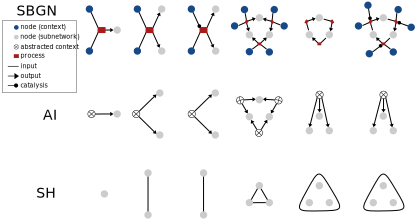
\includegraphics[width=0.9\columnwidth]{fig/netsubnetcontext.pdf}
\caption{{\bf Abstract influence representation of biological networks.} (row~1)~The systems biology graphical notation (SBGN) is capable of representing arbitrary biological networks including processes that involve metabolites, signaling molecules, genes, and enzymes \cite{LeNovere2009}. Only a fragment of the SBGN language, where all nodes have equivalent types, is indicated here. (row~2)~We abstract from the SBGN representation of a biological network to a graph representing the abstract influence (\AI{}) graph indicating coupling among a subset of the entities present in a biological network. (row~3)~For economy of representation we use a short hand (\SH{}) hypergraph to denote the \AI{} graph. The topology of the \AI{} and \SH{} graphs are equivalent and this is what we refer to as network architecture.}
\label{fig:netsubnetcontext}
\end{figure}

\begin{figure}[!ht]
\centering
\noindent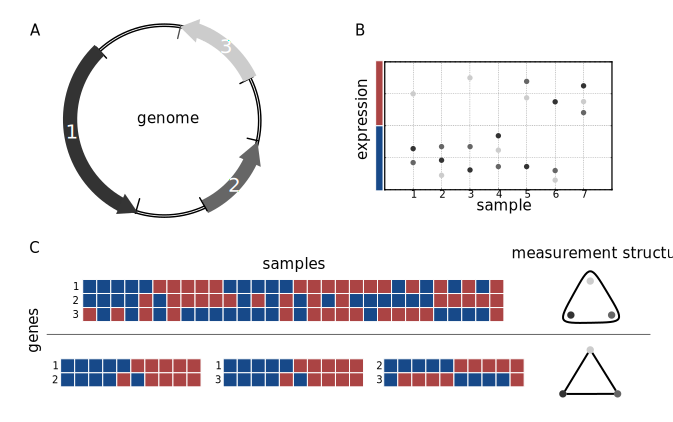
\includegraphics[width=0.9\columnwidth]{fig/figure_expression_concept.pdf}
\caption{{\bf Coarse-graining of biological network data.} (A) SBGN (top) and \SH{} (bottom) representation of two different biological networks. (B) Example binary coarse-graining of biological network data. For each sample a measurement is taken for all three variables in the focal subnetwork. The levels are binned into one of two classes represented by the red---- and blue bars representing relatively high and low levels respectively. (C) Heat map representation of coarse-grained data under the assumption of two different network architectures. The samples on top and the associated measurement structure correspond to the case where constraints are placed on all three variables by a single element of the network context (\ref{fig:stochdynscheme} top row). The bottom represents the case where all three pairs are each independently constrained by elements of the network context (\ref{fig:stochdynscheme} bottom row).}
\label{fig:expression_concept}
\end{figure}

\begin{figure}[!ht]
\centering
\noindent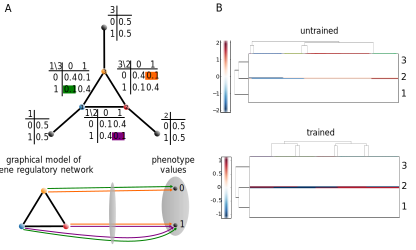
\includegraphics[width=0.9\columnwidth]{fig/inconsistentthreecycle.pdf}
\caption{{\bf Model of inconsistent network state data.} (A) An example structured according to the bottom row of \ref{fig:expression_concept}C. The graph contains three nodes each representing one of the variables depicted in \ref{fig:expression_concept}A. The dashed gray line coming from each variable points to the single variable marginal distribution depicted in the associated table. The pairwise edge marginal distributions are placed along the edges. The highlighted table entries (top) represent the constraint probabilities on the \gnpm{} represented by the equivalently colored arrows (bottom). The binary values representing variable states derive from the coarse-graining process over continuous network state data depicted in \ref{fig:expression_concept}B. (B) Given the model in panel A, the top-left panel represents three hundred samples comprising a data set consistent with a uniform distribution over all \gnpm{}. The top-middle panel represents the joint probability distribution determined via maximum-likelihood estimation with respect to the sufficient statistics (in this case, counts of pairwise observations of variables in states where blue corresponds to 0 and red corresponds to 1) given in the top-left panel. The green bars in the bottom three panels represent the marginalization of this joint distribution according to the structure of the graph. The yellow bars in the bottom three panels represent the ostensible marginal distributions determined via the sum-product algorithm (loopy belief propagation) \cite{Barber2012}. The top-right panel is a schematic where the top gray ellipse represents the space of joint probability distributions on three variables each with two potential states (i.e. $\Delta_7$: the eight-dimensional probability simplex) and the bottom ellipse represents the union of three copies of the four-dimensional probability simplex (i.e. $\Delta_3^{\oplus 3}$), one for each edge in the graph.  For this data, maximum likelihood estimation and loopy belief propagation yield equivalent points in $\Delta_3^{\oplus 3}$. (C) Same as B, but with data consistent with \ref{fig:expression_concept}C bottom, which in the limit of a large amount of data would converge to the ostensible node and edge marginal distributions in panel A. For the given data set, maximum likelihood estimation and loopy belief propagation yield different points in $\Delta_3^{\oplus 3}$.}
\label{fig:inconsistentthreecycle}
\end{figure}

\begin{figure}[!ht]
\centering
\noindent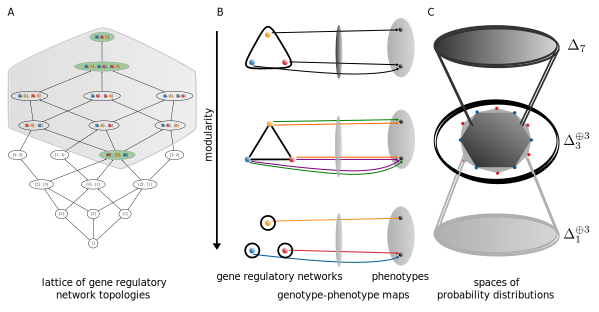
\includegraphics[width=0.9\columnwidth]{fig/conediagram.pdf}
\caption{{\bf Relationship between biological network models and spaces of probability distributions.} (A) The collection of all possible network architectures over three variables forms a lattice represented here by its Hasse diagram. An analogous lattice of network architectures exists for any number of variables. The Hasse diagram shows the manner in which network architectures are hierarchically related and are thus able to be embedded within one another. (B) Explicit examples of \gnpm{} over three network architectures from panel A highlighted in green are represented as arrows mapping the variables represented as nodes of the graph underlying the network architecture into the collection of phenotype values determined by the coarse-graining chosen in \ref{fig:expression_concept}B. There is a different collection of possible \gnpm{} depending upon the structure of the network architecture. (C) Each collection of \gnpm{}, one representative for each network architecture depicted in panel B, is associated to a space of probability distributions defined over it. Moreover, the spaces of probability distributions associated to each graph are related via marginalization maps. The top level represents a joint probability distribution which can be marginalized to the middle space which in turn can be marginalized to the bottom space. The light gray polytope in the middle, $\mathbb{L}(\mathcal{G})$, represents the space of distributions consistent with the marginalization map from the middle to the bottom. The dark gray polytope, $\mathbb{M}(\mathcal{G})$, represents the space of probability distributions consistent with marginalization from the top to the middle.}
\label{fig:conediagram}
\end{figure}

% \begin{figure}[!ht]
% \centering
% \noindent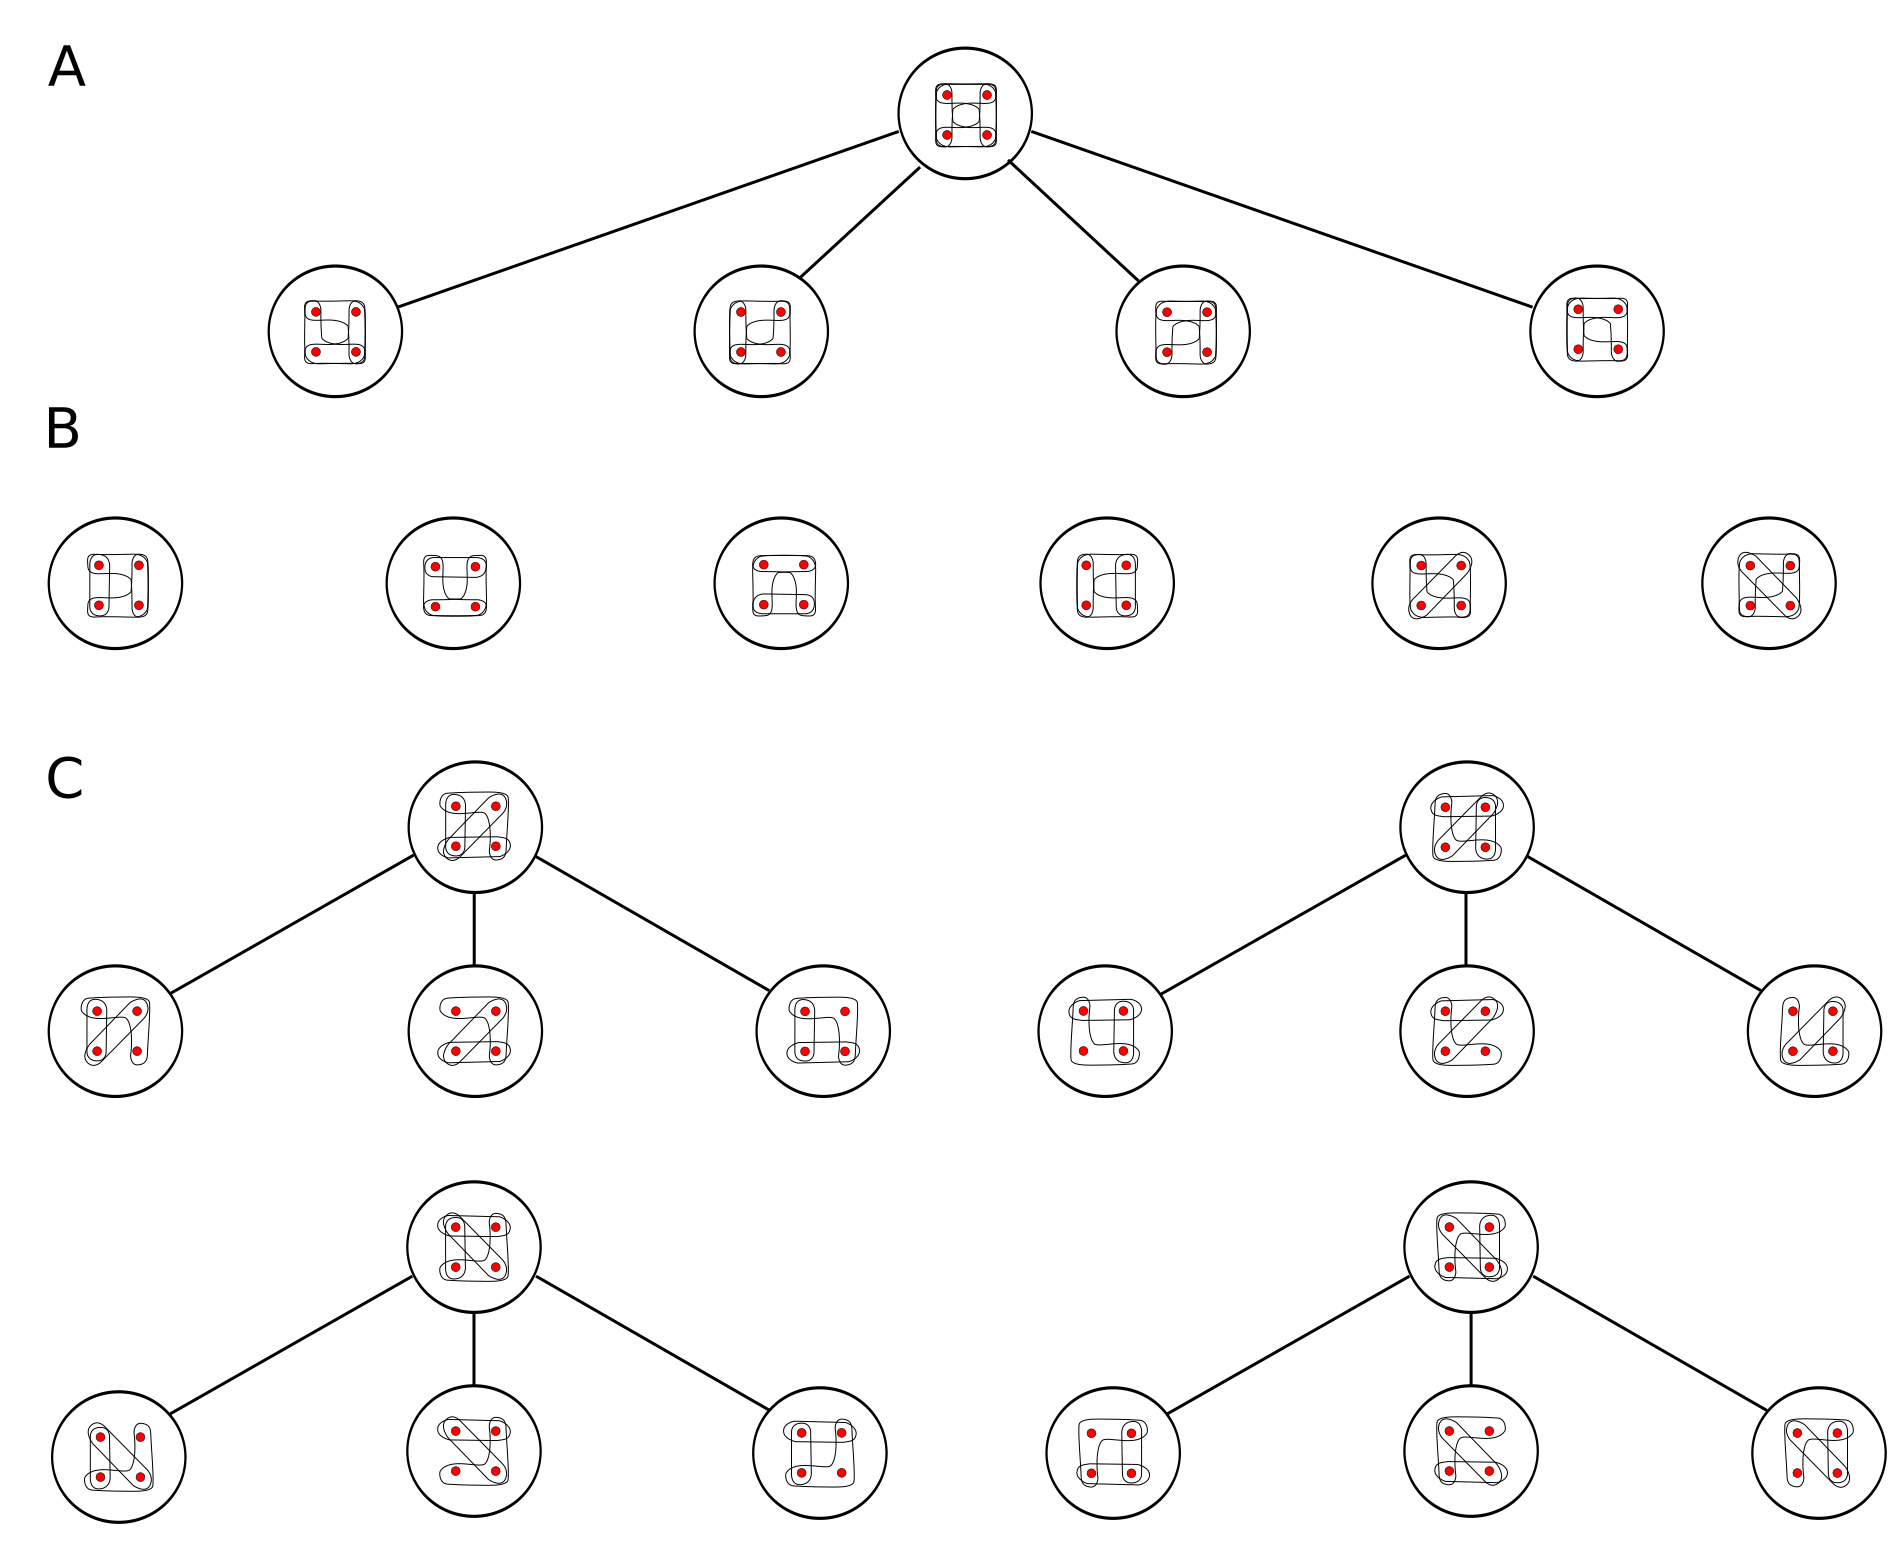
\includegraphics[width=1.0\columnwidth]{fig/non2uniformcyclichypergraphhasse.pdf}
% \caption{{\bf Hierarchical relationships among all possible classes of hypergraphs that are not graphs (i.e. not 2-uniform) but have cycles.} (A) There is a Hasse diagram for the lattice of GRNAs analogous to that of \ref{fig:conediagram}A but defined on four rather than only three genes. Within this lattice some of the graphs have cycles and some do not. (B) The highest levels of the Hasse diagram associated to the lattice of GRNAs on four genes containing hypergraphs having cycles. (C) and (D) contain lower levels of GRNAs containing cycles. Each of the four panels in (D) are on the same level. In total, each level represents an isomorphism class of hypergraphs. Therefore, there are five isomorphism classes of non-2-uniform hypergraphs representing GRNAs on four genes that contain cycles leading to the relationship between spaces of probability distsributions on associated genotype-phentoype maps analogous to that of \ref{fig:conediagram}C.}
% \label{fig:non2uniformcyclichypergraphhasse}
% \end{figure}

\begin{figure}[!ht]
\centering
\noindent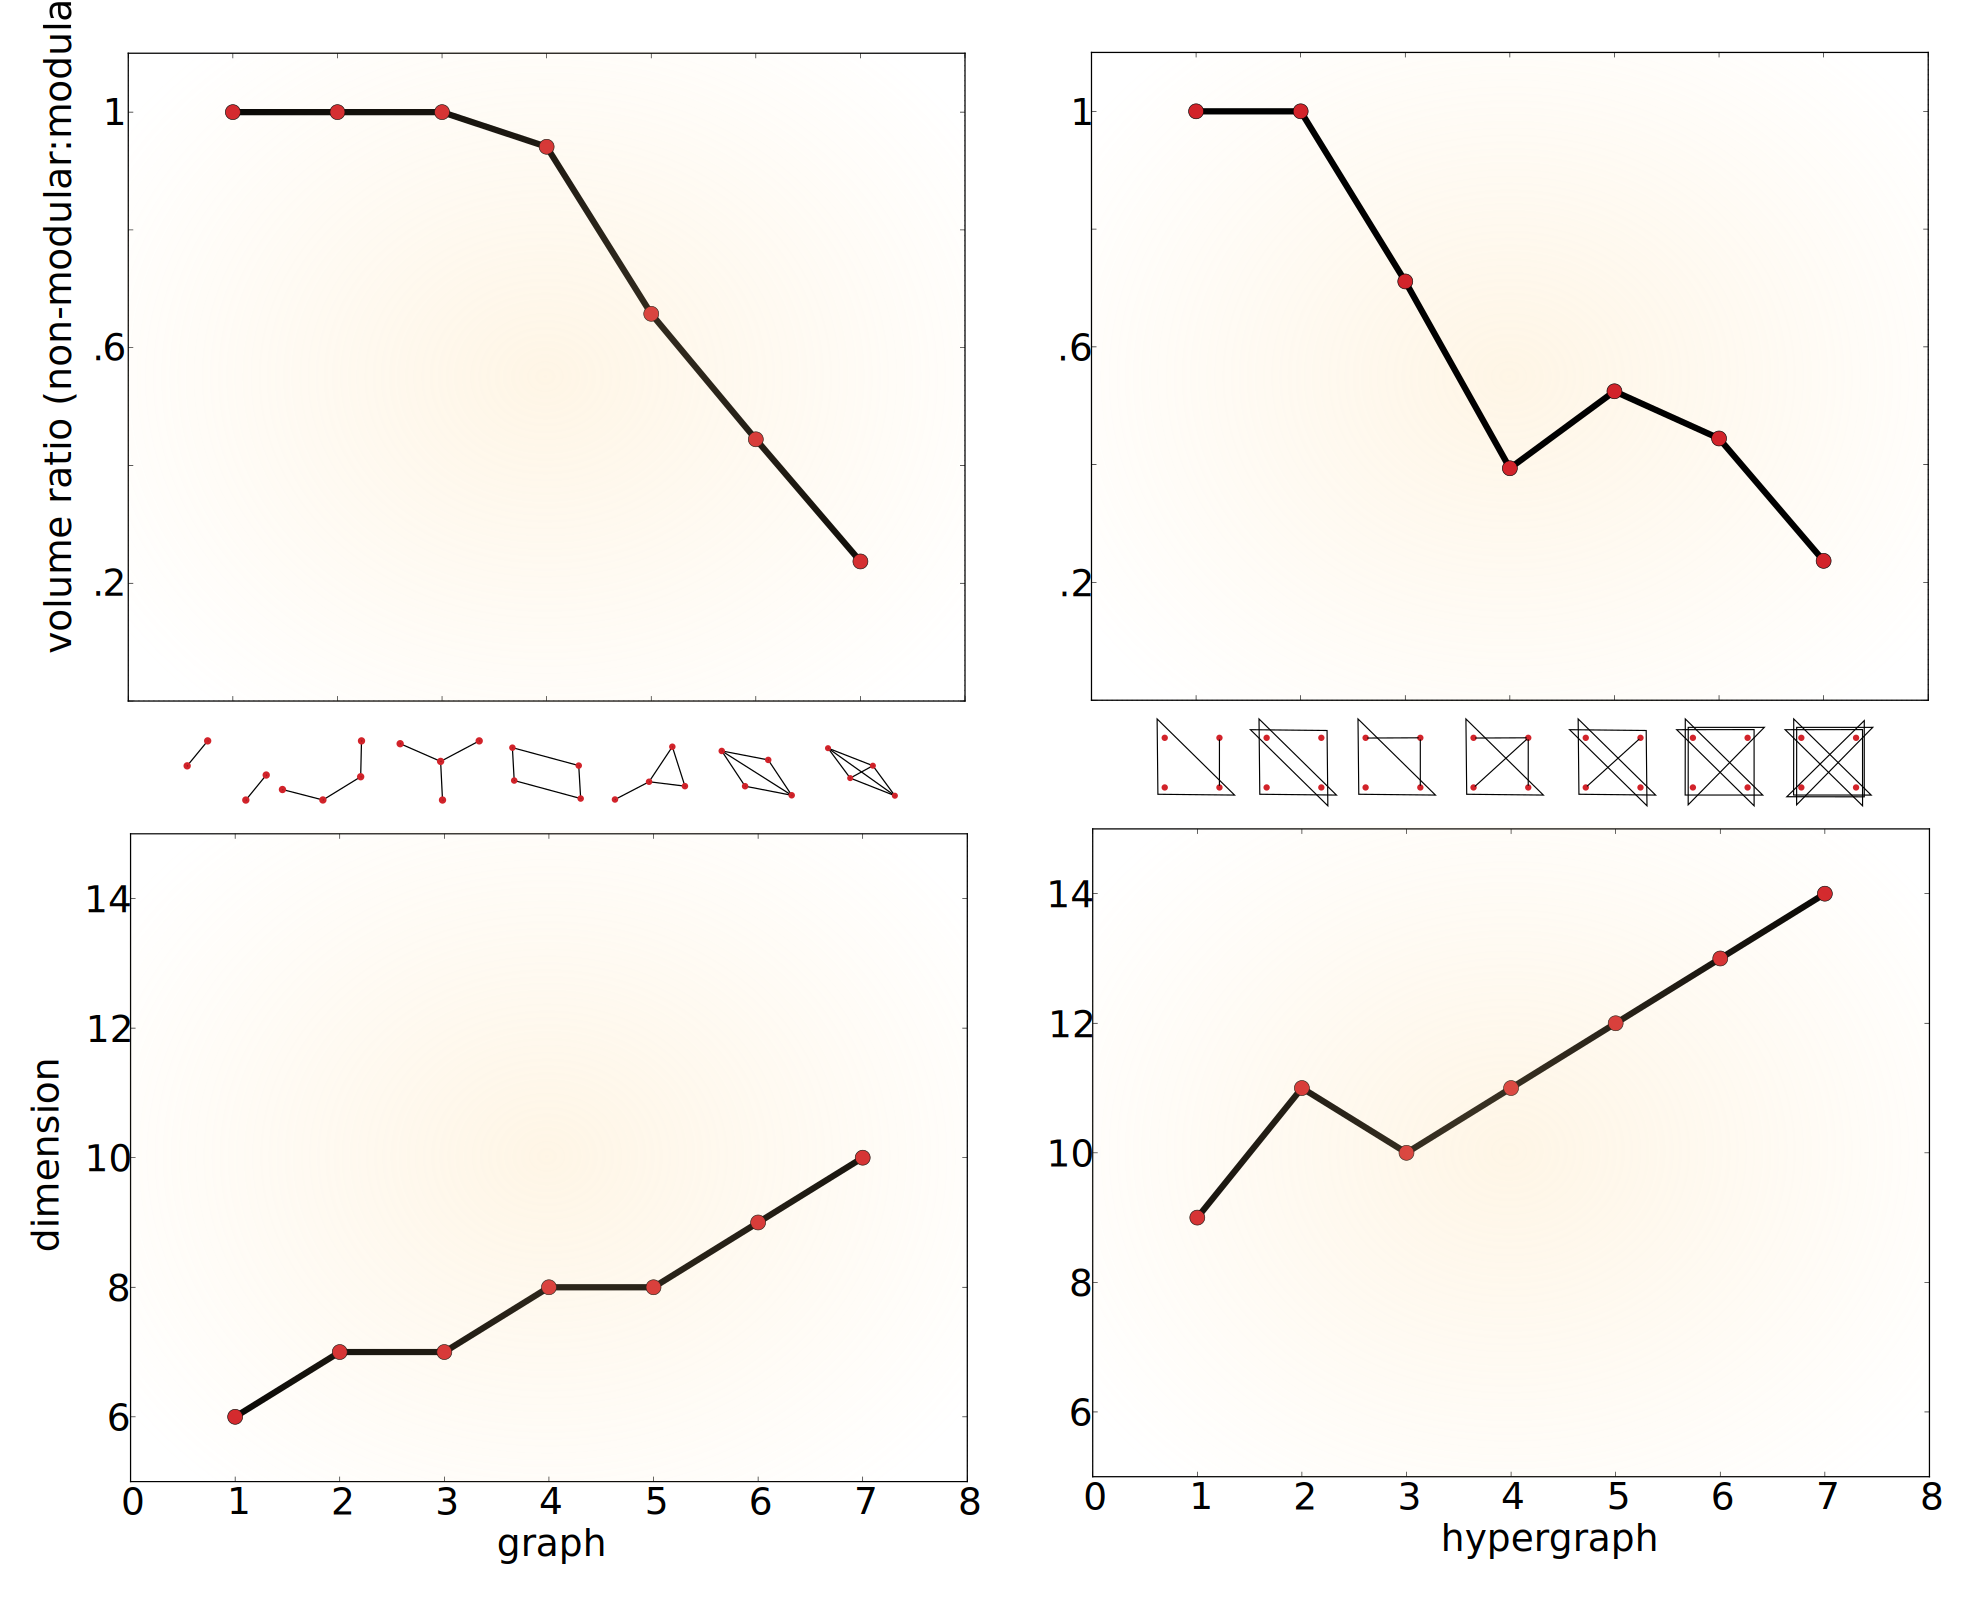
\includegraphics[width=0.9\columnwidth]{fig/figure_graphs_dims_nolines.pdf}
\caption{{\bf Non-modular to modular probability space volume ratio.} (A) and (B) show the ratio $\frac{\text{Vol}(\mathbb{M}(\mathcal{G}))}{\text{Vol}(\mathbb{L}(\mathcal{G}))}$ associated to 2-regular and non-2-regular network architectures respectively. The (hyper)graph associated to each value of the volume ratio is displayed along the x-axis of each panel. (C) and (D) show the natural dimension of the space of probability distributions associated to $\mathbb{M}(\mathcal{G})$ and $\mathbb{L}(\mathcal{G})$ for each hypergraph.}
\label{fig:ncycvolrat}
\end{figure}

\begin{figure}[!ht]
\centering
\noindent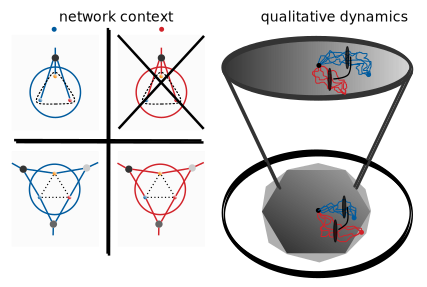
\includegraphics[width=0.9\columnwidth]{fig/stochdynscheme.pdf}
\caption{{\bf Constraints imposed on stochastic biological networks and evolutionary dynamics by network architecture.} Schematic representation of a potential network context (left) for each of the hypothetical stationary probability distributions associated to the fitness peak established by the blue and red points within the spaces of probability distributions represented on the right.
%Algebraically, the top one corresponds to $\dist (\expr (L))$ and the bottom to $\dist (\expr (\mathcal{G}))$.
Either of the two network architectures represented on the left are capable of achieving the stationary distribution over \gnpm{} specified by the blue stationary distribution associated to a hypothetical fitness peak. On the other hand, only the network architecture from the top (and not the bottom) is capable of achieving the red stationary distribution representing an alternative potential fitness peak.}
\label{fig:stochdynscheme}
\end{figure}


\FloatBarrier

%\section{Tables}
%input{tex/table_hidvarmod}
%%!TEX root = ../plos_template.tex
\begin{table}[!ht]
\centering
\begin{subtable}[t]{0.4\textwidth}
\centering
\begin{tabular}{ l || c | c | c | r }
	$L_1 L_2$  &	00 & 01 & 10 & 11\\ \hline
    $l_1 l_2$ & $e_1$ & $e_2$ & $e_3$ & $e_4$\\ \hline
    $l_1 l'_2$ & $e_5$ & $e_6$ & $e_7$ & $e_8$\\ \hline
    $l'_1 l_2$ & $e_9$ & $e_{10}$ & $e_{11}$ & $e_{12}$\\ \hline
    $l'_1 l'_2$ & $e_{13}$ & $e_{14}$ & $e_{15}$ & $e_{16}$\\
    \hline
    \end{tabular}
    \caption{genotype-phenotype maps}
    \label{tab:gpm}
\end{subtable}
~~~~~~
\begin{subtable}[t]{0.4\textwidth}
\centering
	\begin{tabular}{ l || c | c | c | r }
	$L_1 L_2$  &	00 & 01 & 10 & 11\\ \hline
    $l_1 l_2$ & $p_1$ & $p_2$ & $p_3$ & $p_4$\\ \hline
    $l_1 l'_2$ & $p_5$ & $p_6$ & $p_7$ & $p_8$\\ \hline
    $l'_1 l_2$ & $p_9$ & $p_{10}$ & $p_{11}$ & $p_{12}$\\ \hline
    $l'_1 l'_2$ & $p_{13}$ & $p_{14}$ & $p_{15}$ & $p_{16}$\\
    \hline
	\end{tabular}
	\caption{probabilities}
    \label{tab:probabilities}
\end{subtable}
\caption{Genotype-phenotype mapping and associated probability tables for the two locus-two phenotype value example. We use an abbreviated notation in which we use the rewrite rules $l_1 l_2 \rightarrow \{l_1, l_2\}$ and $00 \rightarrow \{0, 0\}$ and all others analogous to avoid an excessive number of brackets.}
\label{tab:example}
\end{table}

%\begin{table}
\centering
\input{tex/table_sheaf_r1}
%!TEX root = ../plos_template.tex
\begin{subtable}[t]{0.4\textwidth}
\centering
\begin{tabular}{ l || c | r }
	$L$  &	0 & 1\\ \hline
    $l_1$ & $p^*_1$ & $p^*_2$\\ \hline
    $l_3$ & \cellcolor{DeepBlue!35} $p^*_3$ & \cellcolor{DeepRed!35} $p^*_4$\\ \hline
    $l_2$ & $p^*_5$ & $p^*_{6}$\\ \hline
    $l_4$ & $p^*_{7}$ & $p^*_{8}$\\
    \hline
    \end{tabular}
    \caption{$l_2$}
    \label{tab:il2}
\end{subtable}
~~~~~~
\begin{subtable}[t]{0.4\textwidth}
\centering
	\begin{tabular}{ l || c | c | c | r }
	$L_1 L_2$  &	00 & 10 & 01 & 11\\ \hline
    $l_1 l_2$ & $p_1$ & $p_2$ & $p_3$ & $p_4$\\ \hline
    $l_1 l_4$ & $p_5$ & $p_6$ & $p_7$ & $p_8$\\ \hline
    $l_3 l_2$ & \cellcolor{DeepBlue!35} $p_9$ & \cellcolor{DeepRed!35} $p_{10}$ & \cellcolor{DeepBlue!35} $p_{11}$ & \cellcolor{DeepRed!35} $p_{12}$\\ \hline
    $l_3 l_4$ & \cellcolor{DeepBlue!35} $p_{13}$ & \cellcolor{DeepRed!35} $p_{14}$ & \cellcolor{DeepBlue!35} $p_{15}$ & \cellcolor{DeepRed!35} $p_{16}$\\
    \hline
	\end{tabular}
	\caption{$l_2$}
    \label{tab:dl2}
\end{subtable}

\begin{subtable}[t]{0.4\textwidth}
\centering
\begin{tabular}{ l || c | r }
	$L$  &	0 & 1\\ \hline
    $l_1$ & $p^*_1$ & $p^*_2$\\ \hline
    $l'_1$ & $p^*_3$ & $p^*_4$\\ \hline
    $l_2$ & \cellcolor{DeepBlue!35} $p^*_5$ & \cellcolor{DeepRed!35} $p^*_{6}$\\ \hline
    $l'_2$ & $p^*_{7}$ & $p^*_{8}$\\
    \hline
    \end{tabular}
    \caption{$l_3$}
    \label{tab:il3}
\end{subtable}
~~~~~~
\begin{subtable}[t]{0.4\textwidth}
\centering
	\begin{tabular}{ l || c | c | c | r }
	$L_1 L_2$  &	00 & 10 & 01 & 11\\ \hline
    $l_1 l_2$ & \cellcolor{DeepBlue!35} $p_1$ & \cellcolor{DeepBlue!35} $p_2$ & \cellcolor{DeepRed!35} $p_3$ & \cellcolor{DeepRed!35} $p_4$\\ \hline
    $l_1 l'_2$ &  $p_5$ & $p_6$ & $p_7$ & $p_8$\\ \hline
    $l'_1 l_2$ & \cellcolor{DeepBlue!35} $p_9$ & \cellcolor{DeepBlue!35} $p_{10}$ & \cellcolor{DeepRed!35} $p_{11}$ & \cellcolor{DeepRed!35} $p_{12}$\\ \hline
    $l'_1 l'_2$ & $p_{13}$ & $p_{14}$ & $p_{15}$ & $p_{16}$\\
    \hline
	\end{tabular}
	\caption{$l_3$}
    \label{tab:dl3}
\end{subtable}

\begin{subtable}[t]{0.4\textwidth}
\centering
\begin{tabular}{ l || c | r }
	$L$  &	0 & 1\\ \hline
    $l_1$ & $p^*_1$ & $p^*_2$\\ \hline
    $l'_1$ & $p^*_3$ & $p^*_4$\\ \hline
    $l_2$ & $p^*_5$ & $p^*_{6}$\\ \hline
    $l'_2$ & \cellcolor{blue!25} $p^*_{7}$ & \cellcolor{green!25} $p^*_{8}$\\    
    \hline
    \end{tabular}
    \caption{$l_4$}
    \label{tab:il4}
\end{subtable}
~~~~~~
\begin{subtable}[t]{0.4\textwidth}
\centering
	\begin{tabular}{ l || c | c | c | r }
	$L_1 L_2$  &	00 & 10 & 01 & 11\\ \hline
    $l_1 l_2$ & $p_1$ & $p_2$ & $p_3$ & $p_4$\\ \hline
    $l_1 l'_2$ & \cellcolor{blue!25} $p_5$ & \cellcolor{blue!25} $p_6$ & \cellcolor{green!20} $p_7$ & \cellcolor{green!20} $p_8$\\ \hline
    $l'_1 l_2$ & $p_9$ & $p_{10}$ & $p_{11}$ & $p_{12}$\\ \hline
    $l'_1 l'_2$ & \cellcolor{blue!25} $p_{13}$ & \cellcolor{blue!25} $p_{14}$ & \cellcolor{green!20} $p_{15}$ & \cellcolor{green!20} $p_{16}$\\
    \hline
	\end{tabular}
	\caption{$l_4$}
    \label{tab:dl4}
\end{subtable}
\caption{Global genotype-phenotype mapping and the sheaf condition for the two-locus-two phenotype value example}
\label{tab:sheaf}
\end{table}
%\begin{table}[!ht]
\centering
\begin{tabular}{ c | l | c }
	\textbf{notation} & \textbf{description} & \textbf{size}\\ \hline \hline
	$\{l_1,l_2\}$ & set of genetic loci & $g = 2$\\ \hline
	$\{a_1,a_2\}$ & set of distinct alleles available to each locus & $a = 2$\\ \hline
	$\{0,1\}$ & set of phenotype values & $p = 2$\\ \hline
	$\{(0,0),(0,1),(1,0),(1,1)\}$ & set of phenotype assignments & $p^g = 4$\\ \hline
	$L = \{l_1,l_2,l'_1,l'_2\}$ & set of all possible alleles for all loci & $ga = 4$\\ \hline
	$\{l_1 l_2,l'_1 l_2,l_1 l'_2,l'_1 l'_2\}$ & set of gene regulatory network modules & $a^g = 4$\\ \hline
$\coprod_{O \in \mathcal{G}} \mathcal{E}(O)$ & set of modularized genotype-phenotype maps  & $(ap)^g = 16$\\ \hline
	$\mathcal{E}(L) = P^L$ & set of global genotype-phenotype maps & $p^{ga} = 16$\\
    \end{tabular}
\caption{Summary of concrete parameter values $(g,a,p)$ in terms of abstract notation for $(g=2,a=2,p=2)$. Note that $\{l_1,l_2,l'_1,l'_2\} \equiv \{l_1,l_2\} \times \{a_1,a_2\}$.}
\label{tab:pars222}
\end{table}

%%!TEX root = ../plos_template.tex
\begin{table}[!ht]
\centering
\begin{tabular}{ r || c | c | c | c | c | c | c | c | c | c | c | c | c | c | c | c }
		\begin{sideways}$l_1 l_2 l_3 l_4$\end{sideways} &	\begin{sideways}0000\end{sideways} & \begin{sideways}0010\end{sideways} & \begin{sideways}0001\end{sideways} & \begin{sideways}0011\end{sideways}
			  & \begin{sideways}1000\end{sideways} & \begin{sideways}1010\end{sideways} & \begin{sideways}1001\end{sideways} & \begin{sideways}1011\end{sideways}
			  &	\begin{sideways}0100\end{sideways} & \begin{sideways}0110\end{sideways} & \begin{sideways}0101\end{sideways} & \begin{sideways}0111\end{sideways}
			  &	\begin{sideways}1100\end{sideways} & \begin{sideways}1110\end{sideways} & \begin{sideways}1101\end{sideways} & \begin{sideways}1111\end{sideways}\\ \hline \hline
    $l_1 l_2 \rightarrow 00$ & 1 & 1 & 1 & 1 & 0 & 0 & 0 & 0 & 0 & 0 & 0 & 0 & 0 & 0 & 0 & 0\\ \hline
    $l_1 l_2 \rightarrow 10$ & 0 & 0 & 0 & 0 & 1 & 1 & 1 & 1 & 0 & 0 & 0 & 0 & 0 & 0 & 0 & 0\\ \hline
    $l_1 l_2 \rightarrow 01$ & 0 & 0 & 0 & 0 & 0 & 0 & 0 & 0 & 1 & 1 & 1 & 1 &  0 & 0 & 0 & 0\\ \hline
    $l_1 l_2 \rightarrow 11$ & 0 & 0 & 0 & 0 & 0 & 0 & 0 & 0 & 0 & 0 & 0 & 0 & 1 & 1 & 1 & 1\\ \hline

    $l_3 l_2 \rightarrow 00$ & 1 & 0 & 1 & 0 & 1 & 0 & 1 & 0 & 0 & 0 & 0 & 0 & 0 & 0 & 0 & 0\\ \hline
    $l_3 l_2 \rightarrow 10$ & 0 & 1 & 0 & 1 & 0 & 1 & 0 & 1 & 0 & 0 & 0 & 0 & 0 & 0 & 0 & 0\\ \hline
    $l_3 l_2 \rightarrow 01$ & 0 & 0 & 0 & 0 & 0 & 0 & 0 & 0 & 1 & 0 & 1 & 0 & 1 & 0 & 1 & 0\\ \hline
    $l_3 l_2 \rightarrow 11$ & 0 & 0 & 0 & 0 & 0 & 0 & 0 & 0 & 0 & 1 & 0 & 1 & 0 & 1 & 0 & 1\\ \hline

    $l_1 l_4 \rightarrow 00$ & 1 & 1 & 0 & 0 & 0 & 0 & 0 & 0 & 1 & 1 & 0 & 0 & 0 & 0 & 0 & 0\\ \hline
    $l_1 l_4 \rightarrow 10$ & 0 & 0 & 0 & 0 & 1 & 1 & 0 & 0 & 0 & 0 & 0 & 0 & 1 & 1 & 0 & 0\\ \hline
    $l_1 l_4 \rightarrow 01$ & 0 & 0 & 1 & 1 & 0 & 0 & 0 & 0 & 0 & 0 & 1 & 1 & 0 & 0 & 0 & 0\\ \hline
    $l_1 l_4 \rightarrow 11$ & 0 & 0 & 0 & 0 & 0 & 0 & 1 & 1 & 0 & 0 & 0 & 0 & 0 & 0 & 1 & 1\\ \hline

    $l_3 l_4 \rightarrow 00$ & 1 & 0 & 0 & 0 & 1 & 0 & 0 & 0 & 1 & 0 & 0 & 0 & 1 & 0 & 0 & 0\\ \hline
    $l_3 l_4 \rightarrow 10$ & 0 & 1 & 0 & 0 & 0 & 1 & 0 & 0 & 0 & 1 & 0 & 0 & 0 & 1 & 0 & 0\\ \hline
    $l_3 l_4 \rightarrow 01$ & 0 & 0 & 1 & 0 & 0 & 0 & 1 & 0 & 0 & 0 & 1 & 0 & 0 & 0 & 1 & 0\\ \hline
    $l_3 l_4 \rightarrow 11$ & 0 & 0 & 0 & 1 & 0 & 0 & 0 & 1 & 0 & 0 & 0 & 1 & 0 & 0 & 0 & 1\\
    \end{tabular}
\caption{Explicit construction of $\mathbf{G}_{n \times m}$ for the case $L = \{ l_1,l_2,l_3,l_4 \}$, $\mathcal{G} = \{\{l_1,l_2 \},\{l_1,l_4 \},\{l_3,l_2\},\{l_3,l_4\} \}$, $P=\{0,1\}$ and thus $\mathbf{G}_{(2 \cdot 2)^2 \times 2^{2 \cdot 2}} = \mathbf{G}_{16 \times 16}$.}
\label{tab:logmat222}
\end{table}


%\FloatBarrier

\pagebreak
\setcounter{secnumdepth}{4}
\section{Supplementary Material}
%!TEX root = ../plos_template.tex

\section{Gene network-phenotype maps}\label{sec:genenetworkphenmap}
The genotype of an organism has a relatively straightforward definition in terms of the sequence of nucleotides comprising its genome. Phenotypes, on the other hand, can be described at different levels of organization~\cite{Dawkins1982,Stadler2001}. The concept of phenotype was initially defined at the level of macroscopically observable physical characteristics such as shape, size, color, and various combinations thereof~\cite{Johannsen1911}. However, since the advent of molecular biology, the lowest level description of phenotype might be considered to be the dynamic phenomenon that can be described by measuring the transcription states of all genes comprising an organism's genome.  These expression levels of subsets of interacting genes determine which enzymes are produced, thus determining the rate at which metabolic reactions proceed.  These reaction rates constitute the next level of phenotypes.  These in turn determine the higher level phenotypes, ultimately culminating in macroscopic phenotypes.  In order to discuss this notion of phenotypic levels in a more precise way, we develop a formal description of the \gnpm{} that takes into account higher-order correlations among genes as well as evidence that gene expression is either stochastic or is more effectively modeled as such.

\ref{fig:expression_concept}A shows a simplified representation of a plasmid encoding a small gene regulatory network (GRN) whose correlation strengths are not known but are to be derived from observation of the transcription process. The amount of a given transcript present in a cell given in terms of the discrete counts obtained via sequence census methods (e.g. RNA-seq) or relative abundance derived from microarray data can be binned into a smaller number of discrete classes by setting a collection of thresholds on the original data set. If only a single threshold is given, then the data can be binned into two classes depending upon whether or not the original measurement surpasses the given threshold in \ref{fig:expression_concept}B.
The time series that results from such observations can be used to infer various statistics that characterize gene expression such as correlations between pairs of genes. The statistics associated to any higher-level phenotype that is determined by a particular gene expression pattern should be functions of such statistics.

If a large enough number of thresholds is available to distinguish among all possible molecule counts, then this observational protocol becomes complementary to mechanistic models.  There may be several sources for stochasticity in \gnpm{} including small numbers of the causal molecules and products of gene expression as well as environmental fluctuations upon which \gnpm{} are conditioned~\cite{Swain2002,Paulsson2004,Thattai2004,Acar2008a,Lestas2010,Munsky2012,Chalancon2012,Neuert2013,Sanchez2013}. Regardless of the fundamental nature of stochasticity to gene expression, empirically, we observe statistical as opposed to deterministic data, and thus we focus here on stochastic models. For our purposes we assume that we are dealing with a stationary stochastic process. Mathematically, such a model may take the form of a Markov chain whose dynamics are governed by a master equation for probability distributions over molecule counts. For example, in the case of a three gene network, the master equation takes the form
$$
\frac{dP(n_1,n_2,n_3)}{dt} = \sum_{n'_1}\sum_{n'_2}\sum_{n'_3} M^{n_1\,n_2\,n_3}_{n'_1\,n'_2\,n'_3}(k) P(n'_1,n'_2,n'_3)
$$
where $P(n_1,n_2,n_3)$ gives the probability of observing $n_1$, $n_2$, and $n_3$ molecules of each of the three genes respectively and $M(k)$ is a Markov transition rate matrix that depends upon some rate functions $k$ that are determined by the network architecture and the dynamics of the interactions.  The solution to this equation will converge towards  a stationary distribution $P_s$ in the limit of long times. We can then coarse-grain over the molecule counts using a function that maps the states represented by vectors of integers into some other variables. For example, if $n_i$ are positive integers, denoting the latter $\mathbb{Z}^+$, then a function $f \colon \mathbb{Z}^+ \rightarrow \{0,1\}$ that takes any integer less than or equal to some threshold $T \in \mathbb{Z}^+$ to $0$ and any integer greater than $T$ to $1$ is a very simple example of such a coarse-graining. For this specific form of the coarse-graining function $f$, the coarse-grained stationary probability distribution takes the form
$$
P_s(b_1,b_2,b_3) = \sum_{n_1 \in f^{-1}(b_1)}\sum_{n_2 \in f^{-1}(b_2)}\sum_{n_3 \in f^{-1}(b_3)} P_s(n_1,n_2,n_3),
$$
where $b_1,b_2,b_3 \in \{ 0,1 \}$. It is also possible to consider the case where each gene is coarse-grained according to a different threshold and into a different number of classes.

At the lowest-level of the \gnpm{}, these coarse-grained expression values can be viewed as collectively determining the lowest level in the aforementioned hierarchy of phenotypes. In this way, the data derived from a number of samples of a given network can be described using binary sequences as in \ref{fig:expression_concept}C.  Summarizing this, we will assume that we have a finite set $L$ of genes and a finite set $P$ of coarse-grained expression levels. These expression levels can also be viewed as complementary to promoter states, and, realistically, the number of these is likely to be larger than two \cite{Rieckh2013a}.  Then a possible expression state of our genome is represented by a function $e : L \to P$ and coarse-graining a stationary distribution will lead to a probability distribution on the set $P^L$ of maps from genes to expression states.

\section{Probability distributions over network modules}\label{sec:probabilitydistributionsonnetworks}

In addition to the expression state of the whole genome, we usually will be interested in the expression states of portions of the genome that interact either directly or indirectly.  We will represent these portions as subsets of $L$ and their expression states as functions from these subsets to $P$. If $O \subset L$, let $\expr{}(O)$ denote the set of all possible functions from $O$ to $P$.

% The power set of $L$, which we shall denote as $\mathcal{P}(L)$, can be regarded  as a category~\cite{Lane1998,MacLane1992,Awodey2006,Abramsky2011} in which the objects are subsets of $L$ and morphisms represent inclusion of a smaller subset into a larger superset (i.e. $O \subseteq O' \Rightarrow O \rightarrow O'$).
If we consider the case in which we have two genes $L=\{l_1,l_2\}$ and there are two potential phenotypes, $P=\{0,1\}$, then $\expr$ operates on each of the possible subsets of $L$ (i.e. $\{\}$, $\{l_1\}$, $\{l_2\}$, $\{l_1,l_2\}$) to give spaces of functions containing the possible \gnpm{} as exemplified in \ref{fig:efunctor}. For example, $\mathcal{E}(\{l_1,l_2\}) = \{ e^{12}_{00},e^{12}_{01},e^{12}_{10},e^{12}_{11} \}$ where $e^{12}_{01}(l_1) = 0$ and $e^{12}_{01}(l_2) = 1$. As another example, $\mathcal{E}(\{l_1\}) = \{ e^{1}_{0},e^{1}_{1} \}$ where $e^{1}_{0}(l_1)=0$ and $e^{1}_{1}(l_1)=1$.

Given a finite set $S$, define $\dist(S)$ to be the set of all probability distributions on $S$. Continuing the example above,
$$\mathcal{D}(\mathcal{E}(\{l_1,l_2\})) = \{p^{12}_{00},p^{12}_{01},p^{12}_{10},p^{12}_{11} \mid p^{12}_{00} \geq 0, p^{12}_{01} \geq 0,p^{12}_{10} \geq 0,p^{12}_{11} \geq 0, p^{12}_{00} + p^{12}_{01} + p^{12}_{10} + p^{12}_{11} = 1 \},$$
$$\mathcal{D}(\mathcal{E}(\{l_1\})) = \{p^{1}_{0}, p^{1}_{1} \mid p^{1}_{0} \geq 0, p^{1}_{1} \geq 0, p^{1}_{0}+p^{1}_{1} = 1 \}.$$

If $S$ and $S'$ are finite sets, which in our case will usually be sets of \gnpm{} given by $\mathcal{E}(O)$, then $d \in \dist(S)$ and $d' \in \dist(S')$ are probability distributions. If $f \colon S \to S'$
is an onto map, then $\dist{}(f)$ is defined as marginalization. For example, in case $S=\{ e^{12}_{00}, e^{12}_{01}, e^{12}_{10}, e^{12}_{11} \}$, $S'=\{ e^{1}_{0}, e^{1}_{1} \}$, and $f$ is given by
\begin{equation}
\begin{aligned}
e^{12}_{00} \mapsto e^{1}_{0}\\
e^{12}_{01} \mapsto e^{1}_{0}\\
e^{12}_{10} \mapsto e^{1}_{1}\\
e^{12}_{11} \mapsto e^{1}_{1}
\end{aligned},
\end{equation}
then $\dist{}(f)$ can be represented as a marginalization matrix
\begin{equation}
\begin{pmatrix}
p^{1}_{0}\\
p^{1}_{1}
\end{pmatrix} = \begin{pmatrix}
1 & 1 & 0 & 0\\
0 & 0 & 1 & 1
\end{pmatrix}
\begin{pmatrix}
p^{12}_{00}\\
p^{12}_{01}\\
p^{12}_{10}\\
p^{12}_{11}
\end{pmatrix}.
\end{equation}

\section{Coarse-graining phenotypes}

As described in \ref{sec:genenetworkphenmap} it is also possible to consider phenotypes that derive from coarse-graining lower-level phenotypes. Once this is done, one arrives at probability distributions over network modules like that introduced in \ref{sec:probabilitydistributionsonnetworks}. As a result of this, our conclusions that are formulated in terms of a single level of coarse-graining \gnpm{} also apply to coarse-graining over multiple levels at once despite the fact that the parameters of the relevant probabilistic model are likely to be different.

For a subset of genes $O \subseteq L$, let $\phi_i (O)$ be the set of phenotype values at level $i$, which can be determined from the expression levels of genes in $O$.  Note that $\phi_i (O)$ may be empty if the set $O$ does not contain enough genes to determine the values of any phenotype at level $i$. If $i \le j$, let $\Omega_{ij}(O) : \phi_i(O) \to \phi_j(O)$ be the coarse-graining map which describes how higher level phenotypes are determined from lower level phenotypes.

For example, if our lower level phenotypes for a set of genes $O_1 = \{ l_1,l_2,l_3,l_4 \}$ are given by a set of binary sequences, then the projection of these phenotypes down to the set $O_2 = \{l_3,l_4\}$ followed by mapping to the higher level phenotypes $x=\{01,10\}$ and $y=\{11\}$ is equivalent to first mapping to the higher-level phenotypes $X$ and $Y$ and then projecting down to $O_2$ shown by the equivalent paths from the top-left to the bottom-right in \ref{fig:phenotypehierarchy}A.
Of course, there is an equivalent diagram for the subset $\{ l_1,l_2,l_3 \}$.

\section{Gene regulatory network modules}\label{sec:covergenotypespace}
A gene regulatory network module is represented by a subset of genes, $O \subseteq L$. A gene regulatory network architecture (GRNA) may then be represented by a subset of such modules, $\mathcal{G} \subseteq \mathcal{P}(L)$ that satisfies the following two conditions
\begin{enumerate}
\item $\cup_i O_i = \cup \mathcal{G} = L$,
\item If $O,O' \in \mathcal{G}$ and $O \subseteq O'$ then $O = O'$.
\end{enumerate}
The first condition is just a statement that $\mathcal{G}$ represents a decomposition of the collection of all genes under consideration into subsets and this is why we refer to $\mathcal{G}$ as a collection of gene regulatory network modules. The second condition means simply that we will not consider nested subsets and so we will take for our $O \in \mathcal{G}$ the biggest $O \in \mathcal{G}$ that is not a subset of some other $O' \in \mathcal{G}$. The second condition also implies that if a given subset of genes $O'$ is compatible in a sense to be explained more precisely in what proceeds then any smaller subset of genes $O$ is also compatible.

Mathematically, the two conditions given above state that $\mathcal{G}$ is a \emph{covering} of the set $L$.  This is equivalent to $(L, \mathcal{G})$ being a reduced hypergraph, Sperner family, or clutter over $L$ \cite{Lauritzen1996}.  Coverings $\mathcal{G}$ of the space of genes contain the necessary information to make precise what we heuristically refer to at other points in this paper as modularity in order to cohere with standard terminology in systems biology literature while attempting to submit our own precise interpretation of the relatively colloquial concept.

Given a covering $\mathcal{G}$ of the space of genes, we can consider the higher order phenotypes associated to the elements of $\mathcal{G}$.  For a suitable choice of cover and a suitable level of phenotypes, it may happen that the phenotypes associated to different elements of $\mathcal{G}$ are distinct.  For instance, in the example of \ref{fig:phenotypehierarchy}, if we take $\mathcal{G} = \{O_1, O_2\}$ where $O_1 = \{l_1, l_2, l_3\}$ and $O_2 = \{l_3, l_4\}$, we have $\phi_{i+1}(O_1) = \{u,v\}$ and $\phi_{i+1}(O_2) = \{x,y\}$.  In such a case, if we were to perform one experiment which measured the phenotypes $\{u,v\}$ and another experiment which measured $\{x,y\}$, then the result could be understood as examining the covering $\{O_1, O_2\}$ at phenotype level $i+1$.

\section{Compatibility of distributions on \gnpm{}}\label{sec:compatibilityofgpms}
Given a covering of the space of genes $\mathcal{G}$, a compatible family for $\mathcal{G}$ with respect to $\mathcal{D} \circ \mathcal{E}$ is given by a family of distributions $\{d_O \in \dist (\mathcal{E}(O)) | O \in \mathcal{G}\}$ such that for all $O, O' \in \mathcal{G}$
\begin{eqnarray}\label{eq:sheafcond}
%\forall O \in \mathcal{G} \left[ \exists d_O \in \mathcal{D}_R\mathcal{E}(O) \right],\\
d_O|O \cap O' = d_{O'}|O \cap O'.
\end{eqnarray}
This first set of conditions is later referred to as local consistency. These conditions mean that any two distributions $d_O$ and $d_{O'}$ in the \emph{compatible family} of distributions marginalize to the same disribution over the intersection of $O$ with $O'$. If these constraints are not satisfied, then there is no way to make a consistent assignment of probabilities to the expression states of even a single gene. In this case one of the constraints will be eliminated or gene duplication may allow for the independent satisfaction of both constraints.

If, moreover, this first condition implies the existence of $d \in \mathcal{D}( \mathcal{E}(L))$ such that $d|O = d_O$ for all $O \in \mathcal{G}$ then the system is said to satisfy the global consistency condition.  We will now examine the situation more closely to determine under what circumstances global consistency holds.

For a cover of the genotype space, $\mathcal{G}$, we can construct a matrix, $\mathbf{G}$, representing the relationship, $R = \coprod_{O \in \mathcal{G}} \mathcal{E}(O \subset L) \subseteq \mathcal{E}(L) \times \expr (\mathcal{G})$, between \gnpm{} having as domain particular gene regulatory network modules given by the $O \in \mathcal{G}$ and those global \gnpm{} defined on $L$. We would like to construct the matrix representation of $\mathbf{G}$. In the first factor, $\mathcal{E}(L) = P^L = \{e^{L}_{\vec{j}} | \vec{j} \in P^{|L|}\}$.
%$\{t_1, \ldots t_m\} = \{t_j | t_j \in P^L\}$.
For the second factor, $ \mathcal{E}(\mathcal{G}) = \coprod_{O \in \mathcal{G}} \mathcal{E}(O) = \{e^O_{\vec{i}} | O \in \mathcal{G}, \vec{i} \in P^{|O|} \}$.
%$\{e_1, \ldots e_n\} = \coprod_{O \in \mathcal{G}} \mathcal{E}(O)$.
 So we have two sets of maps, one defined on $P^L$ and the other defined on $\mathcal{E}(O) = P^O$ for each $O \in \mathcal{G}$. This yields a method of specifying the intended relationship that defines $\mathbf{G}$ for all $e^O_{\vec{i}} \in \mathcal{E}(\mathcal{G})$ and $e^{L}_{\vec{j}} \in \mathcal{E}(L)$:
\begin{eqnarray}\label{eq:margmat}
\mathbf{G}(e^O_{\vec{i}},e^L_{\vec{j}}) =
\begin{cases}
1, & e^L_{\vec{j}}|O = e^O_{\vec{i}},\\
0, & \text{otherwise}.
\end{cases}
\end{eqnarray}
This matrix can be viewed as an operator acting via matrix multiplication on distributions
\begin{eqnarray*}
\mathbf{G} \colon \mathcal{D}(\mathcal{E}(L)) &\rightarrow& \mathcal{D}( \mathcal{E}(\mathcal{G})),\\
d &\mapsto& \coprod_{O \in \mathcal{G}} d|O,
\end{eqnarray*}
and thereby taking a global distribution, $\dist (\mathcal{E}(L))$, defined on \gnpm{} whose domain is the full set of genes $L$ into the local distributions, $\dist (\mathcal{E}(\mathcal{G}))$, that are defined relative to gene regulatory network modules contained in a covering of the genotype space $\mathcal{G}$. $\mathbf{G}$ provides a way of determining the distributions on \gnpm{} for a given context (i.e. $\coprod_{O \in \mathcal{G}} d|O$) that can be derived from distributions (i.e. $\mathcal{D} ( \mathcal{E}(L) )$) defined on the global \gnpm{} (i.e. $\mathcal{E}(L)$ as opposed to $\mathcal{E}(O)$). For example, given the covering $\mathcal{G} = \{ \{l_1\}, \{l_2\} \}$ of a set of two genes $L = \{ l_1, l_2 \}$ the associated matrix $\mathbf{G}$ is shown in \ref{fig:efunctor}B.

Combining the marginalization matrix $\mathbf{G}$ with the maps previously defined in \ref{eq:emb} the following diagram demonstrates the relationships between the spaces of probability distributions and the linear spaces in which they are embedded

\begin{equation*}
\xymatrix{
 \mathbb{R}^{\mathcal{E}(L)} \ar[r]^{\mathbf{G}} &
   \mathbb{R}^{\mathcal{E}(\mathcal{G})} \\
 \dist (\mathcal{E}(L)) \ar[r]^{\mathbf{G}} \ar@{^{(}->}[u]^{emb_{\mathcal{E}(L)}}& \ar@{^{(}->}[u]_{emb_{\mathcal{E}(\mathcal{G})}}
  \dist (\mathcal{E}(\mathcal{G}))
  }
\end{equation*}
The locally, $\mathbb{L}(\mathcal{G})$, and globally, $\mathbb{M}(\mathcal{G})$, consistent polytopes embedded within $\mathbb{R}^{\mathcal{E}(\mathcal{G})}$ correspond to the spaces of probability distributions satisfying the local and global consistency conditions described above. The globally consistent polytope is a subspace of the locally consistent one. This is because an ostensible inverse to $\mathbf{G}$ is underdetermined and can only be estimated in general (most commonly using the maximum entropy principle). In terms of the diagram $\mathbb{M}(\mathcal{G})$ is given by $\mathbf{G}(emb_{\mathcal{E}(L)}(\mathcal{D}(\mathcal{E}(L))))$ and $\mathbb{L}(\mathcal{G})$ is given by $emb_{\mathcal{E}(\mathcal{G})}(\mathcal{D}(\mathcal{E}(\mathcal{G}))) \cap \mathbf{G}(\mathbb{R}^{\mathcal{E}(L)})$, where
\begin{eqnarray}
emb_{\mathcal{E}(\mathcal{G})}(\mathcal{D}(\mathcal{E}(\mathcal{G}))) &=& \left\{ p^{O}_{\vec{i}} \; \bigg| \; (\forall\, O \in \mathcal{G}) \; (\forall\, \vec{i} \in P^{|O|}) \;\; p^O_{\vec{i}} \geq 0, \; (\forall\, O \in \mathcal{G}) \sum_{\vec{i} \in P^{|O|}} p^{O}_{\vec{i}} = 1 \right\},\\
emb_{\mathcal{E}(L)}(\mathcal{D}(\mathcal{E}(L))) &=& \left\{ p^L_{\vec{i}} \; \bigg| \; (\forall\, \vec{i} \in P^{|L|}) \; p^L_{\vec{i}} \geq 0, \; \sum_{\vec{i} \in P^{|L|}} p^L_{\vec{i}} = 1 \right\}.
\end{eqnarray}
To determine explicit conditions on the probabilities we express these in terms of the fundamental subspaces associated to the linear map $\mathbf{G}$. In order for a vector $v$ to lie in $\mathbf{G}(\mathbb{R}^{\mathcal{E}(L)})$, we must have $v=\mathbf{G}x$ for some $x \in \mathbb{R}^{\mathcal{E}(L)}$.  The cokernel of $\mathbf{G}$ gives the obstructions to this system $v=\mathbf{G}x$ having a solution. In order to eliminate these obstructions, constraints must be imposed on $\mathbb{R}^{\mathcal{E}(\mathcal{G})}$ and these constraints are given precisely via annihilating the cokernel, i.e. $\mathbf{G}(\mathbb{R}^{\mathcal{E}(L)}) = \{ v \; | \; (\forall u \in coker \mathbf{G}) \; u \cdot v = 0\}$.  We then take the appropriate intersection to determine $\mathbb{L}(\mathcal{G})$ by requiring $v \in emb_{\mathcal{E}(\mathcal{G})}(\mathcal{D}(\mathcal{E}(\mathcal{G})))$
\begin{eqnarray}\label{eq:localpolytope}
\mathbb{L}(\mathcal{G}) &=& \{ v \in emb_{\mathcal{E}(\mathcal{G})}(\mathcal{D}(\mathcal{E}(\mathcal{G}))) \; | \; (\forall u \in coker \mathbf{G}) \; u \cdot v = 0\}.
\end{eqnarray}
Since $\mathbf{G}$ is not invertible the equation $v = \mathbf{G}x$ can only be solved up to an element of $ker \mathbf{G}$. $v = \mathbf{G}x$ can thus be solved on a subspace $T$ of $\mathbb{R}^{\mathcal{E}(L)}$ such that $T \oplus ker \mathbf{G} = \mathbb{R}^{\mathcal{E}(L)}$ to yield
\begin{eqnarray}\label{eq:globalpolytope}
\mathbb{M}(\mathcal{G}) &=& \{ v \; | v = \mathbf{G} x,\; (\exists x \in T) \; (\exists y \in emb_{\mathcal{E}(L)}(\mathcal{D}(\mathcal{E}(L))))\; x-y \in ker \mathbf{G})  \}.
\end{eqnarray}
In order to obtain inequalities that define $\mathbb{M}(\mathcal{G})$, Fourier-Motzkin elimination can be used to eliminate $x$ and $y$. Alternatively one can use the fact, \cite{Wainwright2007} proposition 8.3, that $\mathbb{M}(\mathcal{G})$ is given by removing the non-integer vertices from a vertex represntation of $\mathbb{L}(\mathcal{G})$ and the ability to interconvert between vertex and inequality representations to compute the same inequalities as described in the \refsupp{}.

\subsection{Example of unsatisfiable constraints}\label{sec:inconsistency}
We will now exemplify equations and inequalities that need to be satisfied in order to guarantee the sheaf condition for the simple case of three genes that form the simplest nontrivial cycle where inconsistency may arise. Suppose that $L = \{l_1,l_2,l_3\}$, $P = \{0,1\}$, $\mathcal{G} = \{\{l_1,l_2\},\{l_2,l_3\},\{l_3,l_1\}\}$. We define probabilities associated to the gene network-phenotype maps for any set $S$ as $p^S_{\vec{j}}= d_{S}(e^S_{\vec{j}})$. This results in $emb_{\mathcal{E}(L)}(\mathcal{D}(\mathcal{E}(L))) = \Delta_7 \subset \mathbb{R}^8 $ and $emb_{\mathcal{E}(\mathcal{G})}(\mathcal{D}(\mathcal{E}(\mathcal{G}))) = \Delta^{\oplus 3}_3 \subset \mathbb{R}^{12}$,
which give the inequalities defining $\mathbb{L}(\mathcal{G})$ and $\mathbb{M}(\mathcal{G})$ when substituted into \ref{eq:localpolytope} and \ref{eq:globalpolytope} with the appropriate $\mathbf{G}$ given by \ref{eq:margmat}.

An example of normalized contingency tables that correspond to this model are presented in \ref{fig:inconsistentthreecycle}A.
One local consistency condition in terms of \ref{eq:sheafcond} specifies that for $e_{\{l_1\}} \in \mathcal{E}(\{l_1\})$, which assigns a particular phenotype to the genotype $\{l_1\}$ rather than to an entire gene regulatory network module like $O$ or $O'$, that
\begin{eqnarray}\label{eq:sheafprob}
\dist (\expr( \{ l_1 \} \subset O ) )(d_O)(e_{\{l_1\}}) = \sum_{\substack{ e \in \mathcal{E}(O), \\  e|l_1=e_{\{l_1\}}} } d_O(e) \,\, = \sum_{\substack{ e' \in \mathcal{E}(O'), \\ e'|l_1=e_{\{l_1\}}} } d_{O'}(e') = \dist (\expr( \{ l_1 \} \subset O' ) )(d_{O'})(e_{\{l_1\}})
\end{eqnarray}
This condition means that the probability for gene $l_1$ to be associated to the phenotype given by $e_{\{l_1\}}$ is equivalent in case we marginalize over all the other genes contained in the gene regulatory network modules of which $l_1$ is a component.  \ref{eq:sheafprob} reduces to two equations corresponding to the case when $e_{l_1}$ is the map which sends $l_1$ to $0$ and the case when $e_{l_1}$ sends $l_1$ to $1$. If we do likewise with $l_2$ and $l_3$ in place of $l_1$ we obtain the set of local consistency conditions:
\begin{equation}
\begin{aligned}\label{eq:localconsistencythreegenes}
 p^{12}_{00} + p^{12}_{01} &= p^{1}_0 = p^{13}_{00} + p^{13}_{01}, &
 p^{12}_{00} + p^{12}_{10} &= p^{2}_0 = p^{23}_{00} + p^{23}_{01}, &
 p^{13}_{00} + p^{13}_{10} &= p^{3}_0 = p^{23}_{00} + p^{23}_{10},\\
 p^{12}_{10} + p^{12}_{11} &= p^{1}_1 = p^{13}_{10} + p^{13}_{11}, &
 p^{12}_{01} + p^{12}_{11} &= p^{2}_1 = p^{23}_{10} + p^{23}_{11}, &
 p^{13}_{01} + p^{13}_{11} &= p^{3}_1 = p^{23}_{01} + p^{23}_{11}.
 \end{aligned}
 \end{equation}
These are equivalent to what would result from using the cokernel of $\mathbf{G}$ in \ref{eq:localpolytope}.
Using the local consistency conditions for our example we can derive a set of inequalities that determine $\mathbb{L}(\mathcal{G})$
\begin{equation}
\begin{aligned}\label{eq:threecycinequalities}
p^{12}_{00} &= 1 + p^{12}_{11} - p^{23}_{10} - p^{23}_{11} - p^{13}_{10} - p^{13}_{11} \geq 0, \\
p^{12}_{01} &= -p^{12}_{11} + p^{23}_{10} + p^{23}_{11} \geq 0,\\
p^{12}_{10} &= -p^{12}_{11} + p^{13}_{10} + p^{13}_{11} \geq 0,\\
p^{23}_{00} &= 1-p^{23}_{10} - p^{13}_{01} - p^{13}_{11} \geq 0,\\
p^{23}_{01} &= -p^{23}_{11} + p^{13}_{01} + p^{13}_{11} \geq 0,\\
p^{31}_{00} &= 1-p^{13}_{10} - p^{13}_{01} - p^{13}_{11} \geq 0,
\end{aligned}
\end{equation}
combined with the trivial inequalities that force all probabilities to be nonnegative. Substituting the numbers from \ref{fig:inconsistentthreecycle}A into \ref{eq:threecycinequalities}, demonstrates that the local conditions are satisfied.

The global consistency conditions form an underdetermined system of linear equations for the putative global distribution $d_{L}$ so their solution will assume the form of a linear subspace as demonstrated in \ref{eq:globalpolytope}.  In our example where this linear subspace corresponds to the image of $\Delta_7$ in $\Delta_3^{\oplus 3}$ under the marginalization map, following \ref{eq:globalpolytope} we can choose $v=p^0_{\vec{i}}$, $y=p^L_{\vec{i}}$, and $T$ by fixing $p^{123}_{000}=0$ we get the following by eliminating $x$ from the equations determined by the conditions $v=Gx$, $x \in T$, $x-y \in ker \mathbf{G}$:
\begin{equation}
\begin{aligned}\label{eq:globalpositivityeqs}
p^{123}_{001} &= p^{12}_{00} - p^{123}_{000} \\
p^{123}_{010} &= p^{13}_{00} - p^{123}_{000} \\
p^{123}_{100} &= p^{23}_{00} - p^{123}_{000} \\
p^{123}_{110} &= p^{23}_{10} - p^{13}_{00} + p^{123}_{000} \\
p^{123}_{011} &= p^{13}_{01} - p^{12}_{00} + p^{123}_{000} \\
p^{123}_{101} &= p^{12}_{10} - p^{23}_{00} + p^{123}_{000} \\
p^{123}_{111} &= 1 - p^{12}_{00} - p^{13}_{00} - p^{23}_{00} - p^{123}_{000}
\end{aligned}
\end{equation}
The remaining condition $y \in emb_{\mathcal{E}(L)}(\mathcal{D}(\mathcal{E}(L)))$ from \ref{eq:globalpolytope} states that all the probabilities $p^{123}_{ijk}$ must be positive numbers, which is only possible if the putative marginals satisfy suitable inequalities given by
\begin{equation}
\begin{aligned}\label{eq:globalpositivityineqs}
p^{123}_{000} &\geq min(p^{12}_{00},\, p^{13}_{00},p^{23}_{00},\, 1 - p^{12}_{00} - p^{13}_{00} - p^{23}_{00}),\\
 p^{123}_{000} &\geq max(0,\, p^{13}_{00}-p^{23}_{10},\, p^{12}_{00}-p^{13}_{01},\, p^{23}_{00}-p^{12}_{10}).
\end{aligned}
\end{equation}
A minimal set of inequalities is then expressed by substituting the equalities from \ref{eq:threecycinequalities} into the inequalities determined by \ref{eq:globalpositivityineqs} and eliminating redundancies resulting in
\begin{equation}
\begin{aligned}\label{eq:threecycbooleinequalities}
p^{12}_{11} - p^{23}_{11} + p^{13}_{01} \geq 0, \\
1 + p^{12}_{11} - p^{23}_{10} - p^{13}_{10} - p^{13}_{01} - p^{13}_{11} \geq 0, \\
-p^{12}_{11} + p^{23}_{10} + p^{13}_{11} \geq 0, \\
-p^{12}_{11} + p^{23}_{11} + p^{13}_{10} \geq 0.
\end{aligned}
\end{equation}
The inequalities from \ref{eq:threecycinequalities} and \ref{eq:threecycbooleinequalities} combined with the nonnegativity inequalities together determine the global polytope $\mathbb{M}(\mathcal{G})$. For the example given in \ref{fig:inconsistentthreecycle}A, the first of the inequalities in \ref{eq:threecycbooleinequalities} is demonstrated to be unsatisfied in \ref{eq:threecycboolenumbers}
\begin{equation}
\begin{aligned}\label{eq:threecycboolenumbers}
0.1 - 0.4 + 0.1 \not\geq 0, \\
1 + 0.1 - 0.1 - 0.1 - 0.1 - 0.4 \geq 0, \\
-0.1 + 0.1 + 0.4 \geq 0, \\
-0.1 + 0.4 + 0.1 \geq 0.
\end{aligned}
\end{equation}
This indicates that data consistent with \ref{fig:inconsistentthreecycle}A could not derive from the network depicted there.
\subsection{Example of apparent satisfaction of unsatisfiable constraints}\label{sec:apparentinconsistency}
The inequalities defining $\mathbb{M}(\mathcal{G})$ were derived under the assumption that the two-element probabilities were obtained by mariginalizing a three-element distribution.  If some other procedure, such as conditionalization, is used to obtain them instead, these inequalities need not apply. For example, suppose now that $L = \{l_1,l_2,l_3 \}$, $P = \{0,1,2\}$, $\mathcal{G} = \{\{l_1,l_2\},\{l_2,l_3\},\{l_3,l_1\}\}$ where we have simply added an element to $P$ relative to the example described above. In the previous example the marginal maps were given by $\dist (\expr (O \subset L))$ with one for each $O \in \mathcal{G}$. If we combine these marginal maps with conditioning on one out of the three genes being in state two and each of the other two being in states zero or one, then we have instead $\dist (\pi_1), \dist (\pi_2), \dist (\pi_3)$ where $\pi_1 = \expr (\{l_1,l_2\} \subset L)|\{ e^{123}_{ij2} \mid i,j \in \{ 0,1 \} \},\; \pi_2 = \expr (\{l_2,l_3\} \subset L)|\{ e^{123}_{2ij} \mid i,j \in \{ 0,1 \} \},\; \pi_3 = \expr (\{l_3,l_1\} \subset L)|\{ e^{123}_{i2j} \mid i,j \in \{ 0,1 \} \}$. In this case, if we have the following assignment of probabilities for a distribution $d$
\begin{equation}\label{eq:condprobs}
\begin{aligned}
p^{123}_{002} &= 1/30 & p^{123}_{020} &= 2/15 & p^{123}_{200} &= 2/15\\
p^{123}_{012} &= 2/15 & p^{123}_{021} &= 1/30 & p^{123}_{201} &= 1/30\\
p^{123}_{102} &= 2/15 & p^{123}_{120} &= 1/30 & p^{123}_{210} &= 1/30\\
p^{123}_{112} &= 1/30 & p^{123}_{121} &= 2/15 & p^{123}_{211} &= 2/15
\end{aligned}
\end{equation}
with all other probabilities being zero, then $\dist (\pi_1)(d), \dist (\pi_2)(d), \dist (\pi_3)(d)$ are equivalent to the probability tables in \ref{fig:inconsistentthreecycle}A, which as shown in \ref{sec:inconsistency}, could not be achieved by marginalization alone. For example, given that $dom(\pi_1) = \{ e^{123}_{002}, e^{123}_{012}, e^{123}_{102}, e^{123}_{112} \}$ then $d(dom(\pi_1)) = \frac{1}{30} + \frac{2}{30} + \frac{2}{30} + \frac{1}{30} = \frac{1}{3}$. Substituting this factor and the fact that ${\pi_1}^{-1}(e^{12}_{ij}) = e^{123}_{ij2}$ into \ref{eq:distfunctor}
$$
p^{12}_{ij} = \dist (\pi_1)(d)(e^{12}_{ij}) = \frac{d({\pi_1}^{-1}(e^{12}_{ij}))}{d(dom(\pi_1))} = 3 p^{123}_{ij2},
$$
then renormalizes probabilities resulting in $p^{12}_{00} = 0.1, p^{12}_{01} = 0.4, p^{12}_{10} = 0.4, p^{12}_{11} = 0.1$ along with the analogs for $p^{23}_{ij}$ and $p^{13}_{ij}$, which are precisely equivalent to what appears in \ref{fig:inconsistentthreecycle}A as suggested above.

If constraints consistent with those of \ref{fig:inconsistentthreecycle}A are placed on the given network, either the network must add another gene in order to satisfy them directly or the network context imposing those constraints must coarse-grain the network in a suitable way. In what follows, we argue that the former is much more plausible than the latter. This ultimately suggests conditions in which cycle breakage via gene duplication may be selected for to relieve inconsistent constraints that can arise when cycles are present.

%%!TEX root = ../plos_template.tex
\subsection{Constraint deduction method to derive H-representation of $\mathbb{L}(\mathcal{G})$}
The equalities derived by computing the cokernel of the matrix $\mathcal{G}$ given in \autoref{tab:logmat222} and adjoining rows that enforce the normalization of the marginal distributions are represented as a matrix in \autoref{eq:eqmat}.
\begin{equation}\label{eq:eqmat}
\begin{aligned}
\begin{bmatrix}
  -1 & -1 & 0 & 0 & 1 & 1 & 0 & 0 & 0 & 0 & 0 & 0 & 0 & 0 & 0 & 0 & 0\\
  0 & 0 & -1 & -1 & 0 & 0 & 1 & 1 & 0 & 0 & 0 & 0 & 0 & 0 & 0 & 0 & 0\\
  -1 & 0 & -1 & 0 & 0 & 0 & 0 & 0 & 1 & 1 & 0 & 0 & 0 & 0 & 0 & 0 & 0\\
  0 & -1 & 0 & -1 & 0 & 0 & 0 & 0 & 0 & 0 & 1 & 1 & 0 & 0 & 0 & 0 & 0\\
  0 & 0 & 0 & 0 & 0 & 0 & 0 & 0 & -1 & 0 & -1 & 0 & 1 & 1 & 0 & 0 & 0\\
  0 & 0 & 0 & 0 & -1 & 0 & -1 & 0 & 0 & 0 & 0 & 0 & 1 & 0 & 1 & 0 & 0\\
  -1 & -1 & -1 & -1 & 1 & 0 & 1 & 0 & 1 & 0 & 1 & 0 & -1 & 0 & 0 & 1 & 0\\
  1 & 1 & 1 & 1 & 0 & 0 & 0 & 0 & 0 & 0 & 0 & 0 & 0 & 0 & 0 & 0 & 1\\
  0 & 0 & 0 & 0 & 1 & 1 & 1 & 1 & 0 & 0 & 0 & 0 & 0 & 0 & 0 & 0 & 1\\
  0 & 0 & 0 & 0 & 0 & 0 & 0 & 0 & 1 & 1 & 1 & 1 & 0 & 0 & 0 & 0 & 1\\
  0 & 0 & 0 & 0 & 0 & 0 & 0 & 0 & 0 & 0 & 0 & 0 & 1 & 1 & 1 & 1 & 1\\
\end{bmatrix}
\end{aligned}
\end{equation}
The final column represents the right-hand side of each equality. It turns out all but one of the normalization conditions is linearly dependent with respect to the other equalities and so we can reduce this set of $7+4=11$ constraints to the $8$ represented again in matrix form in \autoref{eq:kceqsrefa}.
\begin{equation}\label{eq:kceqsrefa}
\begin{aligned}
\begin{bmatrix}
  1 & 0 & 0 & -1 & 0 & 0 & 1 & 1 & 0 & 0 & 1 & 1 & 0 & 0 & 0 & 0 & 1\\
  0 & 1 & 0 & 1 & 0 & 0 & 0 & 0 & 0 & 0 & -1 & -1 & 0 & 0 & 0 & 0 & 0\\
  0 & 0 & 1 & 1 & 0 & 0 & -1 & -1 & 0 & 0 & 0 & 0 & 0 & 0 & 0 & 0 & 0\\
  0 & 0 & 0 & 0 & 1 & 0 & 1 & 0 & 0 & 0 & 0 & 0 & 0 & 1 & 0 & 1 & 1\\
  0 & 0 & 0 & 0 & 0 & 1 & 0 & 1 & 0 & 0 & 0 & 0 & 0 & -1 & 0 & -1 & 0\\
  0 & 0 & 0 & 0 & 0 & 0 & 0 & 0 & 1 & 0 & 1 & 0 & 0 & 0 & 1 & 1 & 1\\
  0 & 0 & 0 & 0 & 0 & 0 & 0 & 0 & 0 & 1 & 0 & 1 & 0 & 0 & -1 & -1 & 0\\
  0 & 0 & 0 & 0 & 0 & 0 & 0 & 0 & 0 & 0 & 0 & 0 & 1 & 1 & 1 & 1 & 1\\
\end{bmatrix}
\end{aligned}
\end{equation}
These equalities can now be substituted into the positivity inequalities necessary to define any space of probability distributions. This yields a set of inequalities \autoref{eq:polrepindineqs} that specify an H-representation of the polytope $\mathbb{L}(\mathcal{G})$. This is the modular polytope, which is a subspace of $\Delta_3^{\times 4}$ associated to distributions consistent with the linear transformation $\mathbf{G}$
\begin{equation}\label{eq:polrepindineqs}
\begin{aligned}
\begin{bmatrix}
  1 & 1 & -1 & -1 & -1 & -1 & 0 & 0 & 0\\
  0 & -1 & 0 & 0 & 1 & 1 & 0 & 0 & 0\\
  0 & -1 & 1 & 1 & 0 & 0 & 0 & 0 & 0\\
  1 & 0 & -1 & 0 & 0 & 0 & -1 & 0 & -1\\
  0 & 0 & 0 & -1 & 0 & 0 & 1 & 0 & 1\\
  1 & 0 & 0 & 0 & -1 & 0 & 0 & -1 & -1\\
  0 & 0 & 0 & 0 & 0 & -1 & 0 & 1 & 1\\
  1 & 0 & 0 & 0 & 0 & 0 & -1 & -1 & -1\\
  0 & 1 & 0 & 0 & 0 & 0 & 0 & 0 & 0\\
  0 & 0 & 1 & 0 & 0 & 0 & 0 & 0 & 0\\
  0 & 0 & 0 & 1 & 0 & 0 & 0 & 0 & 0\\
  0 & 0 & 0 & 0 & 1 & 0 & 0 & 0 & 0\\
  0 & 0 & 0 & 0 & 0 & 1 & 0 & 0 & 0\\
  0 & 0 & 0 & 0 & 0 & 0 & 1 & 0 & 0\\
  0 & 0 & 0 & 0 & 0 & 0 & 0 & 1 & 0\\
  0 & 0 & 0 & 0 & 0 & 0 & 0 & 0 & 1\\
\end{bmatrix}
\end{aligned}
\end{equation}
A row $(a_0,a_1,...,a_d)$ corresponds to the inequality $a_0 + a_1 x_1 + ... + a_d x_d >= 0$. The embedded identity matrix has, in this particular case eight, rows that specify the positivity of the variables corresponding to each of the, in this particular case eight, dimensions. Transforming this inequality or H-representation to a vertex or V-representation of the modular polytope produces \autoref{eq:vrepfromhrep}.
\begin{equation}\label{eq:vrepfromhrep}
\begin{aligned}
\begin{bmatrix}
  1 & 0 & 0 & 0 & 0 & 0 & 0 & 0 & 1\\
  1 & 0 & 0 & 0 & 0 & 0 & 0 & 1 & 0\\
  1 & 0 & 0 & 0 & 0 & 0 & 1 & 0 & 0\\
  1 & 1/2 & 1/2 & 0 & 1/2 & 0 & 1/2 & 1/2 & 0\\
  1 & 1/2 & 0 & 1/2 & 0 & 1/2 & 1/2 & 1/2 & 0\\
  1 & 0 & 0 & 0 & 0 & 0 & 0 & 0 & 0\\
  1 & 1/2 & 1/2 & 0 & 0 & 1/2 & 0 & 0 & 1/2\\
  1 & 1/2 & 0 & 1/2 & 1/2 & 0 & 0 & 0 & 1/2\\
  1 & 0 & 0 & 1/2 & 0 & 1/2 & 0 & 0 & 1/2\\
  1 & 0 & 1/2 & 0 & 1/2 & 0 & 0 & 0 & 1/2\\
  1 & 0 & 1/2 & 0 & 0 & 1/2 & 1/2 & 1/2 & 0\\
  1 & 0 & 0 & 1/2 & 1/2 & 0 & 1/2 & 1/2 & 0\\
  1 & 1 & 1 & 0 & 1 & 0 & 0 & 0 & 0\\
  1 & 0 & 0 & 0 & 1 & 0 & 0 & 0 & 0\\
  1 & 0 & 1 & 0 & 0 & 0 & 0 & 0 & 0\\
  1 & 0 & 0 & 1 & 0 & 0 & 1 & 0 & 0\\
  1 & 0 & 0 & 0 & 0 & 1 & 0 & 1 & 0\\
  1 & 0 & 0 & 0 & 1 & 0 & 1 & 0 & 0\\
  1 & 0 & 1 & 0 & 0 & 0 & 0 & 1 & 0\\
  1 & 1 & 0 & 1 & 0 & 1 & 0 & 0 & 1\\
  1 & 1 & 0 & 1 & 1 & 0 & 1 & 0 & 0\\
  1 & 1 & 1 & 0 & 0 & 1 & 0 & 1 & 0\\
  1 & 0 & 0 & 1 & 0 & 0 & 0 & 0 & 1\\
  1 & 0 & 0 & 0 & 0 & 1 & 0 & 0 & 1\\
\end{bmatrix}
\end{aligned}
\end{equation}
This completes steps 1 and 2 of the algorithm outlined in the previous section. The remaining steps 3 through 5 are trivial. They are simply represented in the Appendices containing the code that implements them.

%%!TEX root = ../plos_template.tex
\subsection{Vertex enumeration method to derive V-representation}
We, therefore, follow Ara\'{u}jo {\it et al.} \cite{Araujo2012} in transforming from probability to expectation value coordinates which allow us to express the coordinates of the vertices of the polytopes corresponding to the joint distributions on non-modular genotype-phenotype mappings, $\Delta_{15}$, and the marginal distributions on modular genotype-phenotype mappings, $\Delta_3^{\otimes 4}$, in a manner that intrinsically enforces normalization and Kolmogorov consistency. Positivity of the probability coordinates can then be enforced via inequalities that result from the transformation from probability to expected value coordinates.

The transformation employs the so-called Hadamard matrix. The Hadamard matrix $H$ of order $n$ has entries in the set $\{+1,-1\}$ and is defined recursively such that all rows have zero inner product and are thus orthogonal:
\begin{equation}
\begin{aligned}\label{eq:hadamard}
H_1 &= [1]\\
H_2 &= \begin{bmatrix}
1 & 1\\
1 & -1
\end{bmatrix}\\
H_{2^k} &= \begin{bmatrix}
H_{2^{k-1}} & H_{2^{k-1}}\\
H_{2^{k-1}} & -H_{2^{k-1}}
\end{bmatrix}
\end{aligned}
\end{equation}
For the gene regulatory network module given by $\{l_1,l_2\}$, we can describe the transformation of coordinates from the probabilities $\vec{p}_{l_1 l_2} = (p_1, p_2, p_3, p_4)$ to the expectation values $\vec{E}_{l_1 l_2} = (1, \langle l_1 \rangle, \langle l_2 \rangle, \langle l_1 l_2 \rangle)$ using the Hadamard matrix $H_{2k}$ for $k=2$ as
\begin{equation}
\begin{aligned}\label{eq:expecttrans}
H_4 \vec{p}_{l_1 l_2} = \vec{E}.
\end{aligned}
\end{equation}
Since the inverse of the Hadamard transform is proportional to itself (i.e. $H_{2k}^{-1} = \frac{1}{2k}H_{2k}$) we can solve this system of equations to express each probability parameter in terms of expected value coordinates
\begin{equation}
\begin{aligned}\label{eq:expecttransfull}
\vec{p}_{l_1 l_2} &= H_4^{-1}\vec{E}\\
\begin{bmatrix}
p_1\\
p_2\\
p_3\\
p_4
\end{bmatrix} &= \frac{1}{4}\begin{bmatrix}
  1 & 1 & 1 & 1\\
  1 & -1 & 1 & -1\\
  1 & 1 & -1 & -1\\
  1 & -1 & -1 & 1\\
\end{bmatrix} \begin{bmatrix}
1\\
\langle l_1 \rangle\\
\langle l_2 \rangle\\
\langle l_1 l_2 \rangle
\end{bmatrix}
\end{aligned}
\end{equation}
Recall that these equations enforce normalization and Kolmogorov consistency. We can additionally enforce positivity, $p_i \geq 0$, in terms of the expectation value coordinates as
\begin{equation}
\begin{aligned}\label{eq:kcineq}
\begin{bmatrix}
  1 & 1 & 1 & 1\\
  1 & -1 & 1 & -1\\
  1 & 1 & -1 & -1\\
  1 & -1 & -1 & 1\\
\end{bmatrix} \begin{bmatrix}
1\\
\langle l_1 \rangle\\
\langle l_2 \rangle\\
\langle l_1 l_2 \rangle
\end{bmatrix} &\geq \begin{bmatrix}
0\\
0\\
0\\
0
\end{bmatrix}\\
H_4^{-1}\vec{E} &\geq \vec{0}
\end{aligned}
\end{equation}
Analogous equations hold for all other gene regulatory network modules given by $\{l'_1,l_2\}, \{l_1,l'_2\}, \{l'_1,l'_2\}$ yielding a total of $4n$ inequalities. Of these, only $2n$ are independent. Vertices of the polytopes corresponding to both the non-modular and modular spaces of probability distributions in terms of expectation value coordinates are of the form
\begin{equation}
\begin{aligned}\label{eq:expvalvert}
\left( \langle l_1 \rangle, \langle l_2 \rangle, \langle l'_1 \rangle, \langle l'_2 \rangle, \langle l_1 l_2 \rangle, \langle l'_1 l_2 \rangle, \langle l'_1 l'_2 \rangle, \langle l_1 l'_2 \rangle  \right).
\end{aligned}
\end{equation}
In the case at hand it turns out that there are $2^n + 2^{n-1}$ vertices of the polytope corresponding to the space of modular distributions and $2^n$ are strictly non-modular while $2^{n-1}$ are strictly modular. For the $(2,2,2)$ case at hand corresponding to the $4-$cycle graph this gives $24$ vertices for the modular polytope and $16$ vertices for the non-modular polytope. The $2^n$ non-modular vertices are given by
\begin{equation}
\begin{aligned}\label{eq:nonmodvert}
\left( \langle l_1 \rangle, \langle l_2 \rangle, \langle l'_1 \rangle, \langle l'_2 \rangle, \langle l_1 \rangle \langle l_2 \rangle, \langle l'_1 \rangle \langle l_2 \rangle, \langle l'_1 \rangle \langle l'_2 \rangle, \langle l_1 \rangle \langle l'_2 \rangle  \right).
\end{aligned}
\end{equation}
and the $2^{n-1}$ modular vertices are given by
\begin{equation}
\begin{aligned}\label{eq:modvert}
\left( 0, 0, 0, 0, \langle l_1 l_2 \rangle, \langle l'_1 l_2 \rangle, \langle l'_1 l'_2 \rangle, \langle l_1 l'_2 \rangle  \right)
\end{aligned}
\end{equation}
where the $\langle l_i l_{i+1} \rangle$ take values in the set $\{+1,-1\}$ such that there are an odd number of negatives in each of the vertices indicated in \ref{eq:modvert}. To be explicit, this results for the $(2,2,2)$ case of the $4-$cycle graph in the following $2^n + 2^{n-1}$ vertices for the modular polytope
\begin{equation}
\begin{aligned}\label{eq:modvertexp}
\begin{bmatrix}
  -1 & -1 & -1 & -1 & 1 & 1 & 1 & 1\\
  -1 & -1 & -1 & 1 & 1 & 1 & -1 & -1\\
  -1 & -1 & 1 & -1 & 1 & -1 & -1 & 1\\
  -1 & -1 & 1 & 1 & 1 & -1 & 1 & -1\\
  -1 & 1 & -1 & -1 & -1 & -1 & 1 & 1\\
  -1 & 1 & -1 & 1 & -1 & -1 & -1 & -1\\
  -1 & 1 & 1 & -1 & -1 & 1 & -1 & 1\\
  -1 & 1 & 1 & 1 & -1 & 1 & 1 & -1\\
  1 & -1 & -1 & -1 & -1 & 1 & 1 & -1\\
  1 & -1 & -1 & 1 & -1 & 1 & -1 & 1\\
  1 & -1 & 1 & -1 & -1 & -1 & -1 & -1\\
  1 & -1 & 1 & 1 & -1 & -1 & 1 & 1\\
  1 & 1 & -1 & -1 & 1 & -1 & 1 & -1\\
  1 & 1 & -1 & 1 & 1 & -1 & -1 & 1\\
  1 & 1 & 1 & -1 & 1 & 1 & -1 & -1\\
  1 & 1 & 1 & 1 & 1 & 1 & 1 & 1\\
  0 & 0 & 0 & 0 & -1 & 1 & 1 & 1\\
  0 & 0 & 0 & 0 & 1 & -1 & 1 & 1\\
  0 & 0 & 0 & 0 & 1 & 1 & -1 & 1\\
  0 & 0 & 0 & 0 & 1 & 1 & 1 & -1\\
  0 & 0 & 0 & 0 & -1 & -1 & -1 & 1\\
  0 & 0 & 0 & 0 & -1 & -1 & 1 & -1\\
  0 & 0 & 0 & 0 & -1 & 1 & -1 & -1\\
  0 & 0 & 0 & 0 & 1 & -1 & -1 & -1\\
\end{bmatrix}
\end{aligned}
\end{equation}
and $2^n$ vertices for the non-modular polytope
\begin{equation}
\begin{aligned}\label{eq:nonmodvertexp}
\begin{bmatrix}
  -1 & -1 & -1 & -1 & 1 & 1 & 1 & 1\\
  -1 & -1 & -1 & 1 & 1 & 1 & -1 & -1\\
  -1 & -1 & 1 & -1 & 1 & -1 & -1 & 1\\
  -1 & -1 & 1 & 1 & 1 & -1 & 1 & -1\\
  -1 & 1 & -1 & -1 & -1 & -1 & 1 & 1\\
  -1 & 1 & -1 & 1 & -1 & -1 & -1 & -1\\
  -1 & 1 & 1 & -1 & -1 & 1 & -1 & 1\\
  -1 & 1 & 1 & 1 & -1 & 1 & 1 & -1\\
  1 & -1 & -1 & -1 & -1 & 1 & 1 & -1\\
  1 & -1 & -1 & 1 & -1 & 1 & -1 & 1\\
  1 & -1 & 1 & -1 & -1 & -1 & -1 & -1\\
  1 & -1 & 1 & 1 & -1 & -1 & 1 & 1\\
  1 & 1 & -1 & -1 & 1 & -1 & 1 & -1\\
  1 & 1 & -1 & 1 & 1 & -1 & -1 & 1\\
  1 & 1 & 1 & -1 & 1 & 1 & -1 & -1\\
  1 & 1 & 1 & 1 & 1 & 1 & 1 & 1\\
\end{bmatrix}
\end{aligned}
\end{equation}
The $2^{n-1}$ vertices of the modular polytope excluded from the non-modular polytope violate the $2^{n-1}$ Boole inequalities determining some of the facets of the non-modular polytope. To be explicit, there are $2^n + 2^{n-1}$ facets of the non-modular polytope given by the following inequalities
\begin{equation}
\begin{aligned}\label{eq:nonmodineq}
\langle l_1 \rangle - \langle l_2 \rangle - \langle l_1 l_2 \rangle &\geq -1\\
\langle l_1 \rangle + \langle l_2 \rangle + \langle l_1 l_2 \rangle &\geq -1\\
\langle l_1 \rangle - \langle l'_2 \rangle - \langle l_1 l'_2 \rangle &\geq -1\\
\langle l_1 \rangle + \langle l'_2 \rangle + \langle l_1 l'_2 \rangle &\geq -1\\
-\langle l_1 \rangle + \langle l_2 \rangle - \langle l_1 l_2 \rangle &\geq -1\\
-\langle l_1 \rangle - \langle l_2 \rangle + \langle l_1 l_2 \rangle &\geq -1\\
-\langle l_1 \rangle + \langle l'_2 \rangle - \langle l_1 l'_2 \rangle &\geq -1\\
-\langle l_1 \rangle - \langle l'_2 \rangle + \langle l_1 l'_2 \rangle &\geq -1\\
\langle l_2 \rangle + \langle l'_1 \rangle + \langle l'_1 l_2 \rangle &\geq -1\\
\langle l_2 \rangle - \langle l'_1 \rangle - \langle l'_1 l_2 \rangle &\geq -1\\
-\langle l_2 \rangle + \langle l'_1 \rangle - \langle l'_1 l_2 \rangle &\geq -1\\
-\langle l_2 \rangle - \langle l'_1 \rangle + \langle l'_1 l_2 \rangle &\geq -1\\
\langle l'_1 \rangle - \langle l'_2 \rangle - \langle l'_1 l'_2 \rangle &\geq -1\\
\langle l'_1 \rangle + \langle l'_2 \rangle + \langle l'_1 l'_2 \rangle &\geq -1\\
-\langle l'_1 \rangle + \langle l'_2 \rangle - \langle l'_1 l'_2 \rangle &\geq -1\\
-\langle l'_1 \rangle - \langle l'_2 \rangle + \langle l'_1 l'_2 \rangle &\geq -1\\
\langle l_1 l_2 \rangle - \langle l'_1 l_2 \rangle + \langle l'_1 l'_2 \rangle + \langle l_1 l'_2 \rangle &\geq -2\\
\langle l_1 l_2 \rangle + \langle l'_1 l_2 \rangle - \langle l'_1 l'_2 \rangle + \langle l_1 l'_2 \rangle &\geq -2\\
\langle l_1 l_2 \rangle + \langle l'_1 l_2 \rangle + \langle l'_1 l'_2 \rangle - \langle l_1 l'_2 \rangle &\geq -2\\
\langle l_1 l_2 \rangle - \langle l'_1 l_2 \rangle - \langle l'_1 l'_2 \rangle - \langle l_1 l'_2 \rangle &\geq -2\\
-\langle l_1 l_2 \rangle + \langle l'_1 l_2 \rangle - \langle l'_1 l'_2 \rangle - \langle l_1 l'_2 \rangle &\geq -2\\
-\langle l_1 l_2 \rangle - \langle l'_1 l_2 \rangle + \langle l'_1 l'_2 \rangle - \langle l_1 l'_2 \rangle &\geq -2\\
-\langle l_1 l_2 \rangle + \langle l'_1 l_2 \rangle + \langle l'_1 l'_2 \rangle + \langle l_1 l'_2 \rangle &\geq -2\\
-\langle l_1 l_2 \rangle - \langle l'_1 l_2 \rangle - \langle l'_1 l'_2 \rangle + \langle l_1 l'_2 \rangle &\geq -2
\end{aligned}
\end{equation}
For the modular polytope, there are $2^n$ inequalities
\begin{equation}
\begin{aligned}\label{eq:modineq}
\langle l_1 \rangle + \langle l'_2 \rangle + \langle l_1 l'_2 \rangle &\geq -1\\
\langle l_1 \rangle + \langle l_2 \rangle + \langle l_1 l_2 \rangle &\geq -1\\
\langle l_1 \rangle - \langle l'_2 \rangle - \langle l_1 l'_2 \rangle &\geq -1\\
\langle l_1 \rangle - \langle l_2 \rangle - \langle l_1 l_2 \rangle &\geq -1\\
-\langle l_1 \rangle + \langle l_2 \rangle - \langle l_1 l_2 \rangle &\geq -1\\
-\langle l_1 \rangle - \langle l_2 \rangle + \langle l_1 l_2 \rangle &\geq -1\\
-\langle l_1 \rangle - \langle l'_2 \rangle + \langle l_1 l'_2 \rangle &\geq -1\\
-\langle l_1 \rangle + \langle l'_2 \rangle - \langle l_1 l'_2 \rangle &\geq -1\\
\langle l_2 \rangle + \langle l'_1 \rangle + \langle l'_1 l_2 \rangle &\geq -1\\
-\langle l_2 \rangle + \langle l'_1 \rangle - \langle l'_1 l_2 \rangle &\geq -1\\
-\langle l_2 \rangle - \langle l'_1 \rangle + \langle l'_1 l_2 \rangle &\geq -1\\
\langle l_2 \rangle - \langle l'_1 \rangle - \langle l'_1 l_2 \rangle &\geq -1\\
\langle l'_1 \rangle - \langle l'_2 \rangle - \langle l'_1 l'_2 \rangle &\geq -1\\
-\langle l'_1 \rangle + \langle l'_2 \rangle - \langle l'_1 l'_2 \rangle &\geq -1\\
\langle l'_1 \rangle + \langle l'_2 \rangle + \langle l'_1 l'_2 \rangle &\geq -1\\
-\langle l'_1 \rangle - \langle l'_2 \rangle + \langle l'_1 l'_2 \rangle &\geq -1
\end{aligned}
\end{equation}
The modular polytope is thus not required to respect the $2^{n-1}$ Boole inequalities which enables it to possess the $2^{n-1}$ additional vertices specified in \ref{eq:modvertexp} with respect to those specified in \ref{eq:nonmodvertexp}. The relationship between the vertex (V) and facet (H) representation given by the explicit enumeration of vertices \ref{eq:modvertexp} and \ref{eq:nonmodvertexp} and inequalities \ref{eq:modineq} and \ref{eq:nonmodineq} have been verified using polymake \cite{GawrilowEwgenijD-TJoswig2000}.

We can additionally use polymake to compute the volume of each polytope and thus evaluate the relative size of the space of models contained within each of the modular and non-modular polytopes. We can compute this volume and thus compare models for arbitrary $n-$cycle graphs. The volume ratios between the non-modular and modular polytopes were computed using polymake for $n=\{3,4,5,6\}$ and are displayed in Figure \ref{fig:ncycvolrat}.


\FloatBarrier

\begin{table}
\centering
\begin{tabular}{ r || c }
$l_1 l_2 l'_1 l'_2$ & probability \\ \hline
0000 & $q_1$ \\
0010 & $q_2$ \\
0001 & $q_3$ \\
0011 & $q_4$ \\
1000 & $q_5$ \\
1010 & $q_6$ \\
1001 & $q_7$ \\
1011 & $q_8$ \\
0100 & $q_9$ \\
0110 & $q_{10}$ \\
0101 & $q_{11}$ \\
0111 & $q_{12}$ \\
1100 & $q_{13}$ \\
1110 & $q_{14}$ \\
1101 & $q_{15}$ \\
1111 & $q_{16}$
\end{tabular}
\caption{Example of a distribution defined on the collection of maps from the set of all possible alleles, $L$, to the set of phenotype values, $P$. Such a distribution may be an instance of a global section $d \in \mathcal{D}_R\mathcal{E}(L)$ if it satisfies the sheaf condition.  Here each row represents the probability assigned to a map in the collection of maps given by the set $P^L$. For example, $P[l_1=0,l_2=0,l'_1=0,l'_2=0]=q_1$ gives the probability associated to the map $\{l_1, l_2, l'_1, l'_2\} \mapsto \{0,0,0,0\}$.}
\label{tab:hidvarmod}
\end{table}
%!TEX root = ../plos_template.tex
\begin{table}[!ht]
\centering
\begin{subtable}[t]{0.4\textwidth}
\centering
\begin{tabular}{ l || c | c | c | r }
	$L_1 L_2$  &	00 & 01 & 10 & 11\\ \hline
    $l_1 l_2$ & $e_1$ & $e_2$ & $e_3$ & $e_4$\\ \hline
    $l_1 l'_2$ & $e_5$ & $e_6$ & $e_7$ & $e_8$\\ \hline
    $l'_1 l_2$ & $e_9$ & $e_{10}$ & $e_{11}$ & $e_{12}$\\ \hline
    $l'_1 l'_2$ & $e_{13}$ & $e_{14}$ & $e_{15}$ & $e_{16}$\\
    \hline
    \end{tabular}
    \caption{genotype-phenotype maps}
    \label{tab:gpm}
\end{subtable}
~~~~~~
\begin{subtable}[t]{0.4\textwidth}
\centering
	\begin{tabular}{ l || c | c | c | r }
	$L_1 L_2$  &	00 & 01 & 10 & 11\\ \hline
    $l_1 l_2$ & $p_1$ & $p_2$ & $p_3$ & $p_4$\\ \hline
    $l_1 l'_2$ & $p_5$ & $p_6$ & $p_7$ & $p_8$\\ \hline
    $l'_1 l_2$ & $p_9$ & $p_{10}$ & $p_{11}$ & $p_{12}$\\ \hline
    $l'_1 l'_2$ & $p_{13}$ & $p_{14}$ & $p_{15}$ & $p_{16}$\\
    \hline
	\end{tabular}
	\caption{probabilities}
    \label{tab:probabilities}
\end{subtable}
\caption{Genotype-phenotype mapping and associated probability tables for the two locus-two phenotype value example. We use an abbreviated notation in which we use the rewrite rules $l_1 l_2 \rightarrow \{l_1, l_2\}$ and $00 \rightarrow \{0, 0\}$ and all others analogous to avoid an excessive number of brackets.}
\label{tab:example}
\end{table}

\begin{table}
\centering
\input{tex/table_sheaf_r1}
%!TEX root = ../plos_template.tex
\begin{subtable}[t]{0.4\textwidth}
\centering
\begin{tabular}{ l || c | r }
	$L$  &	0 & 1\\ \hline
    $l_1$ & $p^*_1$ & $p^*_2$\\ \hline
    $l_3$ & \cellcolor{DeepBlue!35} $p^*_3$ & \cellcolor{DeepRed!35} $p^*_4$\\ \hline
    $l_2$ & $p^*_5$ & $p^*_{6}$\\ \hline
    $l_4$ & $p^*_{7}$ & $p^*_{8}$\\
    \hline
    \end{tabular}
    \caption{$l_2$}
    \label{tab:il2}
\end{subtable}
~~~~~~
\begin{subtable}[t]{0.4\textwidth}
\centering
	\begin{tabular}{ l || c | c | c | r }
	$L_1 L_2$  &	00 & 10 & 01 & 11\\ \hline
    $l_1 l_2$ & $p_1$ & $p_2$ & $p_3$ & $p_4$\\ \hline
    $l_1 l_4$ & $p_5$ & $p_6$ & $p_7$ & $p_8$\\ \hline
    $l_3 l_2$ & \cellcolor{DeepBlue!35} $p_9$ & \cellcolor{DeepRed!35} $p_{10}$ & \cellcolor{DeepBlue!35} $p_{11}$ & \cellcolor{DeepRed!35} $p_{12}$\\ \hline
    $l_3 l_4$ & \cellcolor{DeepBlue!35} $p_{13}$ & \cellcolor{DeepRed!35} $p_{14}$ & \cellcolor{DeepBlue!35} $p_{15}$ & \cellcolor{DeepRed!35} $p_{16}$\\
    \hline
	\end{tabular}
	\caption{$l_2$}
    \label{tab:dl2}
\end{subtable}

\begin{subtable}[t]{0.4\textwidth}
\centering
\begin{tabular}{ l || c | r }
	$L$  &	0 & 1\\ \hline
    $l_1$ & $p^*_1$ & $p^*_2$\\ \hline
    $l'_1$ & $p^*_3$ & $p^*_4$\\ \hline
    $l_2$ & \cellcolor{DeepBlue!35} $p^*_5$ & \cellcolor{DeepRed!35} $p^*_{6}$\\ \hline
    $l'_2$ & $p^*_{7}$ & $p^*_{8}$\\
    \hline
    \end{tabular}
    \caption{$l_3$}
    \label{tab:il3}
\end{subtable}
~~~~~~
\begin{subtable}[t]{0.4\textwidth}
\centering
	\begin{tabular}{ l || c | c | c | r }
	$L_1 L_2$  &	00 & 10 & 01 & 11\\ \hline
    $l_1 l_2$ & \cellcolor{DeepBlue!35} $p_1$ & \cellcolor{DeepBlue!35} $p_2$ & \cellcolor{DeepRed!35} $p_3$ & \cellcolor{DeepRed!35} $p_4$\\ \hline
    $l_1 l'_2$ &  $p_5$ & $p_6$ & $p_7$ & $p_8$\\ \hline
    $l'_1 l_2$ & \cellcolor{DeepBlue!35} $p_9$ & \cellcolor{DeepBlue!35} $p_{10}$ & \cellcolor{DeepRed!35} $p_{11}$ & \cellcolor{DeepRed!35} $p_{12}$\\ \hline
    $l'_1 l'_2$ & $p_{13}$ & $p_{14}$ & $p_{15}$ & $p_{16}$\\
    \hline
	\end{tabular}
	\caption{$l_3$}
    \label{tab:dl3}
\end{subtable}

\begin{subtable}[t]{0.4\textwidth}
\centering
\begin{tabular}{ l || c | r }
	$L$  &	0 & 1\\ \hline
    $l_1$ & $p^*_1$ & $p^*_2$\\ \hline
    $l'_1$ & $p^*_3$ & $p^*_4$\\ \hline
    $l_2$ & $p^*_5$ & $p^*_{6}$\\ \hline
    $l'_2$ & \cellcolor{blue!25} $p^*_{7}$ & \cellcolor{green!25} $p^*_{8}$\\    
    \hline
    \end{tabular}
    \caption{$l_4$}
    \label{tab:il4}
\end{subtable}
~~~~~~
\begin{subtable}[t]{0.4\textwidth}
\centering
	\begin{tabular}{ l || c | c | c | r }
	$L_1 L_2$  &	00 & 10 & 01 & 11\\ \hline
    $l_1 l_2$ & $p_1$ & $p_2$ & $p_3$ & $p_4$\\ \hline
    $l_1 l'_2$ & \cellcolor{blue!25} $p_5$ & \cellcolor{blue!25} $p_6$ & \cellcolor{green!20} $p_7$ & \cellcolor{green!20} $p_8$\\ \hline
    $l'_1 l_2$ & $p_9$ & $p_{10}$ & $p_{11}$ & $p_{12}$\\ \hline
    $l'_1 l'_2$ & \cellcolor{blue!25} $p_{13}$ & \cellcolor{blue!25} $p_{14}$ & \cellcolor{green!20} $p_{15}$ & \cellcolor{green!20} $p_{16}$\\
    \hline
	\end{tabular}
	\caption{$l_4$}
    \label{tab:dl4}
\end{subtable}
\caption{Global genotype-phenotype mapping and the sheaf condition for the two-locus-two phenotype value example}
\label{tab:sheaf}
\end{table}
%\begin{table}[!ht]
\centering
\begin{tabular}{ c | l | c }
	\textbf{notation} & \textbf{description} & \textbf{size}\\ \hline \hline
	$\{l_1,l_2\}$ & set of genetic loci & $g = 2$\\ \hline
	$\{a_1,a_2\}$ & set of distinct alleles available to each locus & $a = 2$\\ \hline
	$\{0,1\}$ & set of phenotype values & $p = 2$\\ \hline
	$\{(0,0),(0,1),(1,0),(1,1)\}$ & set of phenotype assignments & $p^g = 4$\\ \hline
	$L = \{l_1,l_2,l'_1,l'_2\}$ & set of all possible alleles for all loci & $ga = 4$\\ \hline
	$\{l_1 l_2,l'_1 l_2,l_1 l'_2,l'_1 l'_2\}$ & set of gene regulatory network modules & $a^g = 4$\\ \hline
$\coprod_{O \in \mathcal{G}} \mathcal{E}(O)$ & set of modularized genotype-phenotype maps  & $(ap)^g = 16$\\ \hline
	$\mathcal{E}(L) = P^L$ & set of global genotype-phenotype maps & $p^{ga} = 16$\\
    \end{tabular}
\caption{Summary of concrete parameter values $(g,a,p)$ in terms of abstract notation for $(g=2,a=2,p=2)$. Note that $\{l_1,l_2,l'_1,l'_2\} \equiv \{l_1,l_2\} \times \{a_1,a_2\}$.}
\label{tab:pars222}
\end{table}

%!TEX root = ../plos_template.tex
\begin{table}[!ht]
\centering
\begin{tabular}{ r || c | c | c | c | c | c | c | c | c | c | c | c | c | c | c | c }
		\begin{sideways}$l_1 l_2 l_3 l_4$\end{sideways} &	\begin{sideways}0000\end{sideways} & \begin{sideways}0010\end{sideways} & \begin{sideways}0001\end{sideways} & \begin{sideways}0011\end{sideways}
			  & \begin{sideways}1000\end{sideways} & \begin{sideways}1010\end{sideways} & \begin{sideways}1001\end{sideways} & \begin{sideways}1011\end{sideways}
			  &	\begin{sideways}0100\end{sideways} & \begin{sideways}0110\end{sideways} & \begin{sideways}0101\end{sideways} & \begin{sideways}0111\end{sideways}
			  &	\begin{sideways}1100\end{sideways} & \begin{sideways}1110\end{sideways} & \begin{sideways}1101\end{sideways} & \begin{sideways}1111\end{sideways}\\ \hline \hline
    $l_1 l_2 \rightarrow 00$ & 1 & 1 & 1 & 1 & 0 & 0 & 0 & 0 & 0 & 0 & 0 & 0 & 0 & 0 & 0 & 0\\ \hline
    $l_1 l_2 \rightarrow 10$ & 0 & 0 & 0 & 0 & 1 & 1 & 1 & 1 & 0 & 0 & 0 & 0 & 0 & 0 & 0 & 0\\ \hline
    $l_1 l_2 \rightarrow 01$ & 0 & 0 & 0 & 0 & 0 & 0 & 0 & 0 & 1 & 1 & 1 & 1 &  0 & 0 & 0 & 0\\ \hline
    $l_1 l_2 \rightarrow 11$ & 0 & 0 & 0 & 0 & 0 & 0 & 0 & 0 & 0 & 0 & 0 & 0 & 1 & 1 & 1 & 1\\ \hline

    $l_3 l_2 \rightarrow 00$ & 1 & 0 & 1 & 0 & 1 & 0 & 1 & 0 & 0 & 0 & 0 & 0 & 0 & 0 & 0 & 0\\ \hline
    $l_3 l_2 \rightarrow 10$ & 0 & 1 & 0 & 1 & 0 & 1 & 0 & 1 & 0 & 0 & 0 & 0 & 0 & 0 & 0 & 0\\ \hline
    $l_3 l_2 \rightarrow 01$ & 0 & 0 & 0 & 0 & 0 & 0 & 0 & 0 & 1 & 0 & 1 & 0 & 1 & 0 & 1 & 0\\ \hline
    $l_3 l_2 \rightarrow 11$ & 0 & 0 & 0 & 0 & 0 & 0 & 0 & 0 & 0 & 1 & 0 & 1 & 0 & 1 & 0 & 1\\ \hline

    $l_1 l_4 \rightarrow 00$ & 1 & 1 & 0 & 0 & 0 & 0 & 0 & 0 & 1 & 1 & 0 & 0 & 0 & 0 & 0 & 0\\ \hline
    $l_1 l_4 \rightarrow 10$ & 0 & 0 & 0 & 0 & 1 & 1 & 0 & 0 & 0 & 0 & 0 & 0 & 1 & 1 & 0 & 0\\ \hline
    $l_1 l_4 \rightarrow 01$ & 0 & 0 & 1 & 1 & 0 & 0 & 0 & 0 & 0 & 0 & 1 & 1 & 0 & 0 & 0 & 0\\ \hline
    $l_1 l_4 \rightarrow 11$ & 0 & 0 & 0 & 0 & 0 & 0 & 1 & 1 & 0 & 0 & 0 & 0 & 0 & 0 & 1 & 1\\ \hline

    $l_3 l_4 \rightarrow 00$ & 1 & 0 & 0 & 0 & 1 & 0 & 0 & 0 & 1 & 0 & 0 & 0 & 1 & 0 & 0 & 0\\ \hline
    $l_3 l_4 \rightarrow 10$ & 0 & 1 & 0 & 0 & 0 & 1 & 0 & 0 & 0 & 1 & 0 & 0 & 0 & 1 & 0 & 0\\ \hline
    $l_3 l_4 \rightarrow 01$ & 0 & 0 & 1 & 0 & 0 & 0 & 1 & 0 & 0 & 0 & 1 & 0 & 0 & 0 & 1 & 0\\ \hline
    $l_3 l_4 \rightarrow 11$ & 0 & 0 & 0 & 1 & 0 & 0 & 0 & 1 & 0 & 0 & 0 & 1 & 0 & 0 & 0 & 1\\
    \end{tabular}
\caption{Explicit construction of $\mathbf{G}_{n \times m}$ for the case $L = \{ l_1,l_2,l_3,l_4 \}$, $\mathcal{G} = \{\{l_1,l_2 \},\{l_1,l_4 \},\{l_3,l_2\},\{l_3,l_4\} \}$, $P=\{0,1\}$ and thus $\mathbf{G}_{(2 \cdot 2)^2 \times 2^{2 \cdot 2}} = \mathbf{G}_{16 \times 16}$.}
\label{tab:logmat222}
\end{table}


\FloatBarrier
\pagebreak

%!TEX root = ../plos_template.tex
\subsection{Polymake computation of the non-modular:modular volume ratio of probability distribution polytopes for cyclic hypergraphs on three and four vertices}
\begin{python}
"""
hypergraphvolrat.py

given a hypergraph generate a minimal / full-dimensional representation
of the inequalities definitive of (H-rep) the locally consistent
polytope of probability distributions and compute the ratio of its
volume to that of the corresponding globally consistent polytope
"""
import sys
import numpy as np
import sympy as sp
import subprocess
import re
import itertools
from fractions import Fraction

from graphlist4 import graphdict

def kcfromgraph(edgelist=[(0,1),(1,2),(2,3),(3,0)],
                graphname="graph", pvallist=None,
                printlevel=1):
    """
    input: edgelist = the list of edges of a graph
           pvallength = the number of discrete values each node can take
    output: polrepindineqs - polymake compatible minimal
                              representation
            poldim - expected dimension of the resulting polytope
    """
    maxcliques = map(list, edgelist)

    numnodes = len(set([item for sublist in maxcliques for item in sublist]))

    if pvallist is None:
        pvallist = 2*np.ones(numnodes,dtype=np.int)

    stateindices = itertools.product(*map(range,pvallist))
    columns_states = [list(element) for element in stateindices]

    cliquevals = []
    cliqueids = []
    for clique in maxcliques:
        cliquevaliter = itertools.product(*map(range,
                                         [pvallist[i] for i in clique]))
        for cliqueval in cliquevaliter:
            cliquevals.append(list(cliqueval))
            cliqueids.append(clique)

    normconds = np.zeros((len(maxcliques),len(cliqueids)),dtype=np.int)
    normconds = np.append(normconds, np.ones_like(normconds[:,0])[...,None],1)
    for i,maxclique in enumerate(maxcliques):
        for j,cliqueid in enumerate(cliqueids):
            if maxclique==cliqueid:
                normconds[i,j]=1

    ssmat = np.zeros((len(cliquevals),
                      len(columns_states)),dtype=int)

    for i,(cv,cid) in enumerate(zip(cliquevals,cliqueids)):
        for j,cs in enumerate(columns_states):
            if cv==[cs[k] for k in cid]:
                ssmat[i,j]=1

    # Read ssmat from macaulay file
    # fname = '../macaulay/C4_bin.mat'
    # with open(fname) as f:
    #     next(f)
    #     ssmat = np.array([ map(int,line.split()) for line in f ])

    eqmat = np.asarray(sp.Matrix(ssmat.T).nullspace(simplified=True),
                       dtype=np.int)
    eqmat = np.append(eqmat, np.zeros_like(eqmat[:,0])[...,None],1)
    eqmat = np.vstack((eqmat, normconds))

    kceqsref, ind = sp.Matrix(eqmat).rref(simplified=True)
    kceqsrefs = np.squeeze(np.asarray(kceqsref))
    kceqsrefa = kceqsrefs[~np.all(kceqsrefs == 0, axis=1)]

    im1 = np.arange(kceqsrefa.shape[1])
    mask1 = np.ones(len(im1), dtype=bool)
    mask1[ind] = False

    indineqs = kceqsrefa[:, im1[mask1]]

    polrepindineqs = np.zeros(shape=np.shape(indineqs), dtype=np.int)
    polrepindineqs[:, 1:] = -1*indineqs[:, :-1]
    polrepindineqs[:, 0] = indineqs[:, -1]

    poldim = polrepindineqs.shape[1] - 1

    if printlevel:
        print "KC / sufficient statistics matrix"
        print ssmat
        print ""

        print "Full set of equalities (non-homogeneous rhs for normalization)"
        print eqmat
        print ""

        print "Reduced equalities (non-homogeneous rhs)"
        print kceqsrefa
        print ""

        print "Polymake reduced inequalities (homogeneous rhs in first column)"
        print "Each line describes one linear inequality."
        print "The encoding is as follows: "
        print "(a_0,a_1,...,a_d) is the inequality"
              "a_0 + a_1 x_1 + ... + a_d x_d >= 0."
        print polrepindineqs
        print ""

        print "dimension %d\n" % poldim

    return polrepindineqs, poldim

def bmatrix(a):
    """Returns a LaTeX bmatrix

    :a: numpy array
    :returns: LaTeX bmatrix as a string
    """
    if isinstance(a, np.ndarray):
        if len(a.shape) > 2:
            raise ValueError('bmatrix can at most display two dimensions')
        lines = str(a).replace('[', '').replace(']', '').splitlines()
    elif isinstance(a, str):
        lines = a.splitlines()
    else:
        raise ValueError('wrong input type')
    rv = [r'\begin{bmatrix}']
    rv += ['  ' + ' & '.join(l.split()) + r'\\' for l in lines]
    rv +=  [r'\end{bmatrix}']
    return '\n'.join(rv)

def posineqgen(poldim):
    """
    output: polymake compatibile positivity inequalities
    """
    posineq = np.zeros(shape=(poldim, poldim+1), dtype=np.int)
    posineq[:, 1:] = np.identity(poldim)
    return posineq

def minineqgen(eqfname):
    """
    output: minineqs - combine the Kolmogorov Consistency inequalities
                       with positivity inequalities
    """
    eqmat, poldim = kcfromgraph(graphdict[eqfname],eqfname)
    posmat = posineqgen(poldim)
    minineqs = eqmat.tolist() + posmat.tolist()

    return minineqs, poldim

def runpolymakescript(minineqs, representation, polyproperty, eqfname='graph'):
    """
    intermediate: filestring - polymake script with full-dimensional / minimal
                         H-representation of the Kolmogorov Consistent
                         polytope
    output: polyout - output of polymake for given minineqs and
                      polyproperty
    """
    filestring = str("$Verbose::credits=0;\nuse application "
                     "\"polytope\";\nmy $ndineqs=new "
                     "Matrix<Rational>(%s);\nmy $nd=new "
                     "Polytope<Rational>(%s=>$ndineqs);\nprint "
                     "$nd->%s;" %
                     (str(minineqs), representation, polyproperty))

    scriptname = eqfname + "kcscript.pl"
    fname = open(scriptname,'w')
    fname.write(filestring)
    fname.close()
    polyout = subprocess.check_output(["polymake", "--script",
                                               scriptname])

    return polyout

def booleverts(polyvertices):
    """
    remove rational vertices
    """
    def filtrat(line):
        """
        filter lines with '/'s indicating rational numbers
        """
        if "/" not in line:
            vert = [int(x) for x in line.split(' ')]
            return vert
        else:
            return

    filtverts = [filtrat(line)
                             for line in polyvertices.split('\n')[:-1]]
    filtverts = [l for l in filtverts if l is not None]
    return filtverts

def convert(srat):
    """
    convert rational number string to float
    """
    try:
        return float(srat)
    except ValueError:
        num, denom = srat.split('/')
        return float(num) / float(denom)

def approxvol(minineqs,eqfname,error_threshold=0.2):
    minineqstr = re.sub(r'], ',r'],\n',str(minineqs))

    centroid = list(0.125*np.ones(np.shape(minineqs)[1]-1))
    filestring = str("addpath('volconvbod');\n"
                     "aa=%s;\n"
                     "bb = [aa(:,2:end) aa(:,1)];\n"
                     "bb(:,1:end-1)=-1*bb(:,1:end-1);\n"
                     "intpoint = %s';\n"
                     "Volume(bb,[],%s,intpoint)" %
                     (minineqstr, centroid, error_threshold))
    scriptname = eqfname + "Vol"
    fname = open(scriptname + ".m",'w')
    fname.write(filestring)
    fname.close()

    #matlab -nodesktop -nojvm -nosplash -r "run polymakeVol; exit;"
    matprocout = subprocess.check_output(["matlab", "-nodesktop",
                                      "-nojvm", "-nosplash",
                                      "-logfile", scriptname + ".out",
                                      "-r", scriptname + "; exit;"])
    fname = open(scriptname + ".out")
    matout = fname.read()
    fname.close()
    vollist = re.findall(r'(?<=Final Volume: ).*(?=,)',matout)
    vol = float(vollist[0])
    return vol

def minineqrep(argv):
    """
    usage: python minineqrep.py C4 VERTICES
    """
    eqfname = str(argv[0])
    polyproperty = str(argv[1])

    print "Name of graph: \n%s\n" % eqfname

    minineqs, dim = minineqgen(eqfname)
    polyout = runpolymakescript(minineqs, "INEQUALITIES",
                                polyproperty, eqfname)

    #poutbmatrix = bmatrix(polyout)

    if polyproperty == "VERTICES":
        boolepolyverts = booleverts(polyout)
        volboole = runpolymakescript(boolepolyverts,
                            "POINTS", "VOLUME", eqfname)

        volkolmogorov = runpolymakescript(minineqs,
                                        "INEQUALITIES", "VOLUME", eqfname)
        vrat = convert(volboole) / convert(volkolmogorov)
        #print "%s/%s ~ %0.6f" % (volboole, volkolmogorov, vrat)
        print "Volume of Boole polytope"
        print volboole
        print ""

        print "Volume of Kolmogorov polytope"
        print volkolmogorov
        print ""

        print "Volume ratio Boole:Kolmogorov"
        print vrat
        print ""

    print "Vertices of Kolmogorov polytope\n" + polyout
    return vrat, dim

if __name__ == "__main__":
    minineqrep(sys.argv[1:])
\end{python}

\pagebreak

\subsection{Example graphs on four vertices}
\input{tex/graphlist4}
\pagebreak

\subsection{Generate the lattice of hypergraphs on a given number of vertices}
\input{tex/hypergraphlattice}
\pagebreak

\subsection{Filter hypergraphs with cycles using Graham reduction}
\begin{python}
"""
hypergraphcycle.py

implementation of the Graham reduction method
for hypergraph cycle detection
http://web.cecs.pdx.edu/~maier/TheoryBook/MAIER/C13.pdf#page=18
"""

from copy import deepcopy
import numpy as np
import hypergraph as hg
import hypergraph.core as hgc

def remove_ear(G):
    H = deepcopy(G)
    for v in H.vertices:
        if len(H.incident(v))==1:
            edge_containing_ear = H.incident(v).pop()
            non_ear_vertices = set.difference(set(edge_containing_ear),
                                              set([v]))
            if non_ear_vertices:
                edge_lacking_ear = hgc.Edge(non_ear_vertices)
                edges_lacking_ear = deepcopy(H.edges)
                edges_lacking_ear.remove(edge_containing_ear)
                if any([edge_lacking_ear.issubset(e) for e in edges_lacking_ear]):
                    H.remove_vertex(v)
                else:
                    H.remove_edge(edge_containing_ear)
                    H.add_edge(edge_lacking_ear)
            else:
                H.remove_edge(edge_containing_ear)
            break
    return H

def graham_reduce(G):
    progress_flag = True
    cycle_flag = True
    vertex_counter = 1
    hgstack = [G]
    while progress_flag:
        H = hgstack.pop()
        temp=remove_ear(H)
        if temp.edges:
            if temp==H:
                if vertex_counter > len(G.vertices):
                    progress_flag = False
                    cycle_flag = True
            hgstack.append(temp)
        else:
            progress_flag = False
            cycle_flag = False
        vertex_counter += 1
    return cycle_flag

def testcycle(edgelist,numverts):
    hh=hgc.Hypergraph(vertices=set(range(numverts)))
    for e in edgelist:
        hh.add_edge(hgc.Edge(e))
    return graham_reduce(hh)


# for g in graphlist:
#     #print testcycle(g)
#     hh=hgc.Hypergraph(vertices=set([0,1,2,3]))
#     for e in g:
#         hh.add_edge(hgc.Edge(e))
#     print graham_reduce(hh)
\end{python}

\pagebreak

\subsection{Approximate volume computations}
%!TEX root = ../plos_template.tex
\begin{python}
"""
overfourapproxvol.py

use B. Cousins and S. Vempala, A Cubic Algorithm for Computing Gaussian Volume.
2013. [arXiv:1306.5829](http://arxiv.org/abs/1306.5829v2)
to approximate the volume of the globally consistent polytope for
the case of the overfour graph: overfour = [(0,1,2),(0,1,3),(0,2,3),(1,2,3)]
"""

from minineqrep import *

def approxvol(minineqs,eqfname,error_threshold=0.2):
    minineqstr = re.sub(r'], ',r'],\n',str(minineqs))
    #polyout = runpolymakescript(minineqs,
    #                        "INEQUALITIES", "CENTROID", eqfname)
    #centroid = [float(Fraction(s)) for s in polyout.split()][1:]
    centroid = list(0.125*np.ones(np.shape(minineqs)[1]-1))
    filestring = str("addpath('volconvbod');\n"
                     "aa=%s;\n"
                     "bb = [aa(:,2:end) aa(:,1)];\n"
                     "bb(:,1:end-1)=-1*bb(:,1:end-1);\n"
                     "intpoint = %s';\n"
                     "Volume(bb,[],%s,intpoint)" %
                     (minineqstr, centroid, error_threshold))
    scriptname = eqfname + "Vol"
    fname = open(scriptname + ".m",'w')
    fname.write(filestring)
    fname.close()
    #matlab -nodesktop -nojvm -nosplash -r "run polymakeVol; exit;"
    matprocout = subprocess.check_output(["matlab", "-nodesktop",
                                      "-nojvm", "-nosplash",
                                      "-logfile", scriptname + ".out",
                                      "-r", scriptname + "; exit;"])
    fname = open(scriptname + ".out")
    matout = fname.read()
    fname.close()
    vollist = re.findall(r'(?<=Final Volume: ).*(?=,)',matout)
    vol = float(vollist[0])
    return vol

eqfname = "overfour"
minineqs,dim=minineqgen("overfour")
polyout = runpolymakescript(minineqs, "INEQUALITIES", "VERTICES", "overfour")
boolepolyverts = booleverts(polyout)
volboole = runpolymakescript(boolepolyverts,
                            "POINTS", "VOLUME", eqfname)
volkc = approxvol(minineqs,"overfour",0.01)

#9.17659647818378e-11/3.877906e-10
vol = convert(volboole)/volkc
\end{python}



\end{document}
